\setchapterpreamble[u]{\margintoc}
\chapter{Electrodinámica cuántica}
\labch{Part}

\begin{center}
  \large Todo esto lo he sacado del \cite{Dobdado}
\end{center}
La electrodinámica cuántica (QED) describe la interacción entre electrones (o cualquier otra partícula cargada de spin $1 / 2$ como los muones, quarks, etc) y los fotones, así como las interacciones de las partículas cargadas entre sí. La teoría fue desarrollada por F. Dyson, R. Feynman, J. Schwinger y S. Tomonaga a finales de los años 40 y es la primera teoría cuántica de campos que permitió hacer cálculos de forma consistente. La constante de acoplo de la teoría viene dada por la carga del electrón $e$, o más concretamente, por la constante de estructura fina $\alpha=e^{2} / 4 \pi \hbar c \simeq 1 / 137$ que es una cantidad pequeña y por tanto la teoría permite un desarrollo perturbativo como el que hemos visto en el tema anterior.

En este tema estudiaremos las reglas de Feynman para QED y los principales procesos de interacción.
\section{Lagrangiano clásico e invariancia Gauge}
\section{Cuantización, teoría de perturbaciones y reglas de Feymann}
\section{Reglas de Feynman}
\subsection{Part\'{\i}culas en el estado inicial}
\begin{itemize}
    \item \textbf{Electr\'{o}n (ferm\'{i}on) en el estado inicial:} 
    
    \begin{center}
      

\tikzset{every picture/.style={line width=0.75pt}} %set default line width to 0.75pt        

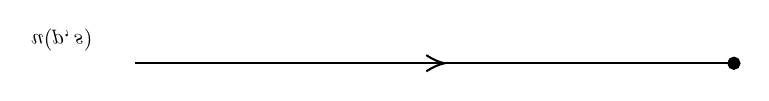
\begin{tikzpicture}[x=0.75pt,y=0.75pt,yscale=-1,xscale=1,scale=0.8, every node/.style={transform shape}]
%uncomment if require: \path (0,32); %set diagram left start at 0, and has height of 32

%Straight Lines [id:da7895899053771676] 
\draw    (153,14) -- (513.71,14) ;
\draw [shift={(513.71,14)}, rotate = 0] [color={rgb, 255:red, 0; green, 0; blue, 0 }  ][fill={rgb, 255:red, 0; green, 0; blue, 0 }  ][line width=0.75]      (0, 0) circle [x radius= 3.35, y radius= 3.35]   ;
\draw [shift={(339.36,14)}, rotate = 180] [color={rgb, 255:red, 0; green, 0; blue, 0 }  ][line width=0.75]    (10.93,-4.9) .. controls (6.95,-2.3) and (3.31,-0.67) .. (0,0) .. controls (3.31,0.67) and (6.95,2.3) .. (10.93,4.9)   ;

% Text Node
\draw (89,8.4) node [anchor=north west][inner sep=0.75pt]    {$u( p,s)$};


\end{tikzpicture}

    \end{center}
    \item \textbf{Positr\'{o}n (antiferm\'{i}on) en el estado inicial:}  \begin{center}
      \tikzset{every picture/.style={line width=0.75pt}}
      
      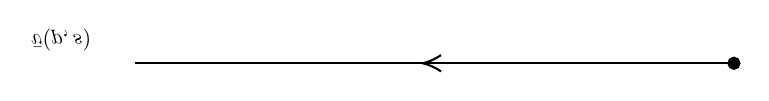
\begin{tikzpicture}[x=0.75pt,y=0.75pt,yscale=-1,xscale=1,scale=0.8, every node/.style={transform shape}]
        %uncomment if require: \path (0,27); %set diagram left start at 0, and has height of 27
        
        %Straight Lines [id:da7895899053771676] 
        \draw    (153,14) -- (513.71,14) ;
        \draw [shift={(513.71,14)}, rotate = 0] [color={rgb, 255:red, 0; green, 0; blue, 0 }  ][fill={rgb, 255:red, 0; green, 0; blue, 0 }  ][line width=0.75]      (0, 0) circle [x radius= 3.35, y radius= 3.35]   ;
        \draw [shift={(326.36,14)}, rotate = 0] [color={rgb, 255:red, 0; green, 0; blue, 0 }  ][line width=0.75]    (10.93,-4.9) .. controls (6.95,-2.3) and (3.31,-0.67) .. (0,0) .. controls (3.31,0.67) and (6.95,2.3) .. (10.93,4.9)   ;
        
        \draw (89,8.4) node [anchor=north west][inner sep=0.75pt]    {$\bar{v}(p,s)$};
        
        
        \end{tikzpicture}
    \end{center}
    \item \textbf{Fot\'{o}n en el estado inicial:}  
    \begin{center}
      

\tikzset{every picture/.style={line width=0.75pt}} %set default line width to 0.75pt        

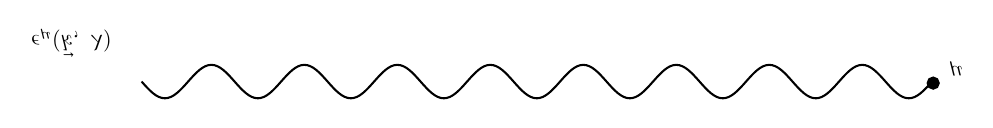
\begin{tikzpicture}[x=0.75pt,y=0.75pt,yscale=-1,xscale=1,scale=0.8, every node/.style={transform shape}]
%uncomment if require: \path (0,45); %set diagram left start at 0, and has height of 45

%Shape: Wave [id:dp44363194459120914] 
\draw   (100,24.93) .. controls (104.57,30.09) and (108.93,35) .. (114,35) .. controls (119.07,35) and (123.43,30.09) .. (128,24.93) .. controls (132.57,19.77) and (136.93,14.86) .. (142,14.86) .. controls (147.07,14.86) and (151.43,19.77) .. (156,24.93) .. controls (160.57,30.09) and (164.93,35) .. (170,35) .. controls (175.07,35) and (179.43,30.09) .. (184,24.93) .. controls (188.57,19.77) and (192.93,14.86) .. (198,14.86) .. controls (203.07,14.86) and (207.43,19.77) .. (212,24.93) .. controls (216.57,30.09) and (220.93,35) .. (226,35) .. controls (231.07,35) and (235.43,30.09) .. (240,24.93) .. controls (244.57,19.77) and (248.93,14.86) .. (254,14.86) .. controls (259.07,14.86) and (263.43,19.77) .. (268,24.93) .. controls (272.57,30.09) and (276.93,35) .. (282,35) .. controls (287.07,35) and (291.43,30.09) .. (296,24.93) .. controls (300.57,19.77) and (304.93,14.86) .. (310,14.86) .. controls (315.07,14.86) and (319.43,19.77) .. (324,24.93) .. controls (328.57,30.09) and (332.93,35) .. (338,35) .. controls (343.07,35) and (347.43,30.09) .. (352,24.93) .. controls (356.57,19.77) and (360.93,14.86) .. (366,14.86) .. controls (371.07,14.86) and (375.43,19.77) .. (380,24.93) .. controls (384.57,30.09) and (388.93,35) .. (394,35) .. controls (399.07,35) and (403.43,30.09) .. (408,24.93) .. controls (412.57,19.77) and (416.93,14.86) .. (422,14.86) .. controls (427.07,14.86) and (431.43,19.77) .. (436,24.93) .. controls (440.57,30.09) and (444.93,35) .. (450,35) .. controls (455.07,35) and (459.43,30.09) .. (464,24.93) .. controls (468.57,19.77) and (472.93,14.86) .. (478,14.86) .. controls (483.07,14.86) and (487.43,19.77) .. (492,24.93) .. controls (496.57,30.09) and (500.93,35) .. (506,35) .. controls (511.07,35) and (515.43,30.09) .. (520,24.93) .. controls (524.57,19.77) and (528.93,14.86) .. (534,14.86) .. controls (539.07,14.86) and (543.43,19.77) .. (548,24.93) .. controls (552.57,30.09) and (556.93,35) .. (562,35) .. controls (567.07,35) and (571.43,30.09) .. (576,24.93) .. controls (576.57,24.28) and (577.14,23.64) .. (577.71,23) ;
%Straight Lines [id:da3953182496879233] 
\draw    (576.71,25.86) ;
\draw [shift={(576.71,25.86)}, rotate = 0] [color={rgb, 255:red, 0; green, 0; blue, 0 }  ][fill={rgb, 255:red, 0; green, 0; blue, 0 }  ][line width=0.75]      (0, 0) circle [x radius= 3.35, y radius= 3.35]   ;

% Text Node
\draw (585,22.83) node [anchor=north west][inner sep=0.75pt]    {$\mu $};
% Text Node
\draw (32,11.83) node [anchor=north west][inner sep=0.75pt]    {$\epsilon _{\mu }(\vec{k} ,\ \lambda )$};


\end{tikzpicture}
\newline
Los $\lambda $ son los 2 estados de polarización del fotón, es decir, $\lambda = 1,2$.
    \end{center}
\end{itemize}

\subsection{Part\'{\i}culas en el estado final}
\begin{itemize}
    \item \textbf{Electr\'{o}n (ferm\'{i}on) en el estado final:} 
    \begin{center}
      

\tikzset{every picture/.style={line width=0.75pt}} %set default line width to 0.75pt        

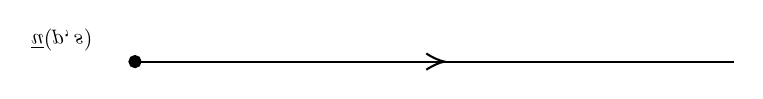
\begin{tikzpicture}[x=0.75pt,y=0.75pt,yscale=-1,xscale=1,scale=0.8, every node/.style={transform shape}]
%uncomment if require: \path (0,32); %set diagram left start at 0, and has height of 32

%Straight Lines [id:da7895899053771676] 
\draw    (153,14) -- (513.71,14) ;
\draw [shift={(339.36,14)}, rotate = 180] [color={rgb, 255:red, 0; green, 0; blue, 0 }  ][line width=0.75]    (10.93,-4.9) .. controls (6.95,-2.3) and (3.31,-0.67) .. (0,0) .. controls (3.31,0.67) and (6.95,2.3) .. (10.93,4.9)   ;
\draw [shift={(153,14)}, rotate = 0] [color={rgb, 255:red, 0; green, 0; blue, 0 }  ][fill={rgb, 255:red, 0; green, 0; blue, 0 }  ][line width=0.75]      (0, 0) circle [x radius= 3.35, y radius= 3.35]   ;

% Text Node
\draw (89,9.4) node [anchor=north west][inner sep=0.75pt]    {$\overline{u}( p,s)$};


\end{tikzpicture}

    \end{center}
    \item \textbf{Positr\'{o}n (antiferm\'{i}on) en el estado final:} \begin{center}
      

\tikzset{every picture/.style={line width=0.75pt}} %set default line width to 0.75pt        

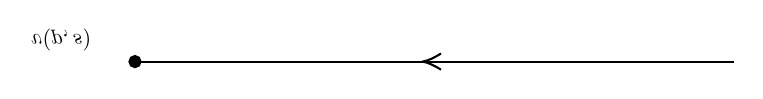
\begin{tikzpicture}[x=0.75pt,y=0.75pt,yscale=-1,xscale=1,scale=0.8, every node/.style={transform shape}]
%uncomment if require: \path (0,32); %set diagram left start at 0, and has height of 32

%Straight Lines [id:da7895899053771676] 
\draw    (153,14) -- (513.71,14) ;
\draw [shift={(326.36,14)}, rotate = 0] [color={rgb, 255:red, 0; green, 0; blue, 0 }  ][line width=0.75]    (10.93,-4.9) .. controls (6.95,-2.3) and (3.31,-0.67) .. (0,0) .. controls (3.31,0.67) and (6.95,2.3) .. (10.93,4.9)   ;
\draw [shift={(153,14)}, rotate = 0] [color={rgb, 255:red, 0; green, 0; blue, 0 }  ][fill={rgb, 255:red, 0; green, 0; blue, 0 }  ][line width=0.75]      (0, 0) circle [x radius= 3.35, y radius= 3.35]   ;

% Text Node
\draw (89,9.4) node [anchor=north west][inner sep=0.75pt]    {$v( p,s)$};


\end{tikzpicture}

    \end{center}
    \item \textbf{Fot\'{o}n en el estado final:} 
    \begin{center}
      

\tikzset{every picture/.style={line width=0.75pt}} %set default line width to 0.75pt        

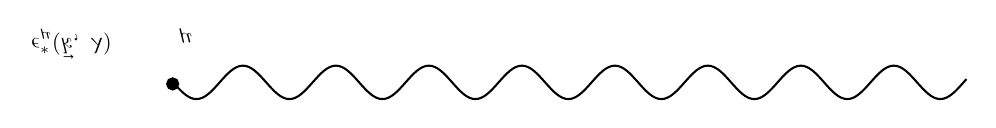
\begin{tikzpicture}[x=0.75pt,y=0.75pt,yscale=-1,xscale=1,scale=0.8, every node/.style={transform shape}]
%uncomment if require: \path (0,45); %set diagram left start at 0, and has height of 45

%Shape: Wave [id:dp44363194459120914] 
\draw   (100,24.93) .. controls (104.57,30.09) and (108.93,35) .. (114,35) .. controls (119.07,35) and (123.43,30.09) .. (128,24.93) .. controls (132.57,19.77) and (136.93,14.86) .. (142,14.86) .. controls (147.07,14.86) and (151.43,19.77) .. (156,24.93) .. controls (160.57,30.09) and (164.93,35) .. (170,35) .. controls (175.07,35) and (179.43,30.09) .. (184,24.93) .. controls (188.57,19.77) and (192.93,14.86) .. (198,14.86) .. controls (203.07,14.86) and (207.43,19.77) .. (212,24.93) .. controls (216.57,30.09) and (220.93,35) .. (226,35) .. controls (231.07,35) and (235.43,30.09) .. (240,24.93) .. controls (244.57,19.77) and (248.93,14.86) .. (254,14.86) .. controls (259.07,14.86) and (263.43,19.77) .. (268,24.93) .. controls (272.57,30.09) and (276.93,35) .. (282,35) .. controls (287.07,35) and (291.43,30.09) .. (296,24.93) .. controls (300.57,19.77) and (304.93,14.86) .. (310,14.86) .. controls (315.07,14.86) and (319.43,19.77) .. (324,24.93) .. controls (328.57,30.09) and (332.93,35) .. (338,35) .. controls (343.07,35) and (347.43,30.09) .. (352,24.93) .. controls (356.57,19.77) and (360.93,14.86) .. (366,14.86) .. controls (371.07,14.86) and (375.43,19.77) .. (380,24.93) .. controls (384.57,30.09) and (388.93,35) .. (394,35) .. controls (399.07,35) and (403.43,30.09) .. (408,24.93) .. controls (412.57,19.77) and (416.93,14.86) .. (422,14.86) .. controls (427.07,14.86) and (431.43,19.77) .. (436,24.93) .. controls (440.57,30.09) and (444.93,35) .. (450,35) .. controls (455.07,35) and (459.43,30.09) .. (464,24.93) .. controls (468.57,19.77) and (472.93,14.86) .. (478,14.86) .. controls (483.07,14.86) and (487.43,19.77) .. (492,24.93) .. controls (496.57,30.09) and (500.93,35) .. (506,35) .. controls (511.07,35) and (515.43,30.09) .. (520,24.93) .. controls (524.57,19.77) and (528.93,14.86) .. (534,14.86) .. controls (539.07,14.86) and (543.43,19.77) .. (548,24.93) .. controls (552.57,30.09) and (556.93,35) .. (562,35) .. controls (567.07,35) and (571.43,30.09) .. (576,24.93) .. controls (576.57,24.28) and (577.14,23.64) .. (577.71,23) ;
%Straight Lines [id:da3953182496879233] 
\draw    (99.71,25.86) ;
\draw [shift={(99.71,25.86)}, rotate = 0] [color={rgb, 255:red, 0; green, 0; blue, 0 }  ][fill={rgb, 255:red, 0; green, 0; blue, 0 }  ][line width=0.75]      (0, 0) circle [x radius= 3.35, y radius= 3.35]   ;

% Text Node
\draw (102,2.83) node [anchor=north west][inner sep=0.75pt]    {$\mu $};
% Text Node
\draw (13,12.83) node [anchor=north west][inner sep=0.75pt]    {$\epsilon _{\mu }^{*}(\vec{k} ,\ \lambda )$};


\end{tikzpicture}
\newline
Los $\lambda $ son los 2 estados de polarización del fotón, es decir, $\lambda = 1,2$.

    \end{center}
\end{itemize}

\subsection{V\'{e}rtice}
\begin{itemize}
    \item \begin{center}
      

\tikzset{every picture/.style={line width=0.75pt}} %set default line width to 0.75pt        

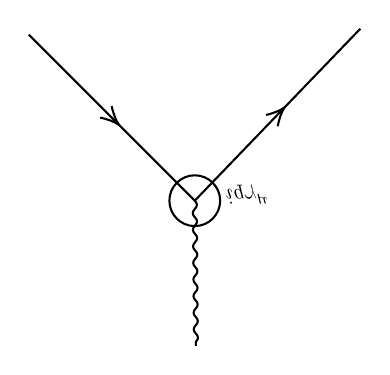
\begin{tikzpicture}[x=0.75pt,y=0.75pt,yscale=-1,xscale=1,scale=0.8, every node/.style={transform shape}]
%uncomment if require: \path (0,213); %set diagram left start at 0, and has height of 213

%Straight Lines [id:da037410651049002874] 
\draw    (228,13) -- (328,113) ;
\draw [shift={(282.24,67.24)}, rotate = 225] [color={rgb, 255:red, 0; green, 0; blue, 0 }  ][line width=0.75]    (10.93,-4.9) .. controls (6.95,-2.3) and (3.31,-0.67) .. (0,0) .. controls (3.31,0.67) and (6.95,2.3) .. (10.93,4.9)   ;
%Straight Lines [id:da8166962722779569] 
\draw    (328,113) -- (427.71,9.43) ;
\draw [shift={(382.02,56.89)}, rotate = 133.91] [color={rgb, 255:red, 0; green, 0; blue, 0 }  ][line width=0.75]    (10.93,-4.9) .. controls (6.95,-2.3) and (3.31,-0.67) .. (0,0) .. controls (3.31,0.67) and (6.95,2.3) .. (10.93,4.9)   ;
%Straight Lines [id:da8632233109264691] 
\draw    (328,113) .. controls (329.68,114.65) and (329.69,116.32) .. (328.04,118) .. controls (326.39,119.68) and (326.4,121.35) .. (328.08,123) .. controls (329.76,124.65) and (329.77,126.32) .. (328.12,128) .. controls (326.47,129.68) and (326.48,131.35) .. (328.16,133) .. controls (329.84,134.65) and (329.85,136.32) .. (328.2,138) .. controls (326.55,139.68) and (326.57,141.35) .. (328.25,143) .. controls (329.93,144.65) and (329.94,146.32) .. (328.29,148) .. controls (326.64,149.68) and (326.65,151.35) .. (328.33,153) .. controls (330.01,154.65) and (330.02,156.32) .. (328.37,158) .. controls (326.72,159.68) and (326.73,161.35) .. (328.41,163) .. controls (330.09,164.65) and (330.1,166.32) .. (328.45,168) .. controls (326.8,169.68) and (326.81,171.35) .. (328.49,173) .. controls (330.17,174.65) and (330.18,176.32) .. (328.53,178) .. controls (326.88,179.68) and (326.89,181.35) .. (328.57,183) .. controls (330.25,184.65) and (330.26,186.32) .. (328.61,188) .. controls (326.96,189.68) and (326.97,191.35) .. (328.65,193) .. controls (330.33,194.65) and (330.34,196.32) .. (328.69,198) -- (328.71,200.43) -- (328.71,200.43) ;

%Shape: Circle [id:dp8472577663241367] 
\draw   (312.71,113) .. controls (312.71,104.56) and (319.56,97.71) .. (328,97.71) .. controls (336.44,97.71) and (343.29,104.56) .. (343.29,113) .. controls (343.29,121.44) and (336.44,128.29) .. (328,128.29) .. controls (319.56,128.29) and (312.71,121.44) .. (312.71,113) -- cycle ;

% Text Node
\draw (345.29,116.4) node [anchor=north west][inner sep=0.75pt]    {$iq \gamma ^{\mu }$};


\end{tikzpicture}
\newline
$q$ (que no es el $q$ del momento de fotón) es 
\begin{DispWithArrows}[format=c, displaystyle]
q=eQ_f \text{ con }Q_f\left\{\begin{array}{c}
  Q_{e,\mu ,\tau }=-1 \\
  Q_{u,c,t }=\frac{2}{3} \\
  Q_{d,s,b}=-\frac{1}{3} \\
\end{array}\right.
\end{DispWithArrows}
    \end{center}
\end{itemize}



\subsection{L\'{\i}neas internas}
\begin{itemize}
    \item \textbf{Propagador fermi\'{o}nico:} \begin{center}
      

\tikzset{every picture/.style={line width=0.75pt}} %set default line width to 0.75pt        

\begin{tikzpicture}[x=0.75pt,y=0.75pt,yscale=-1,xscale=1,scale=0.8, every node/.style={transform shape}]
%uncomment if require: \path (0,69); %set diagram left start at 0, and has height of 69

%Straight Lines [id:da7895899053771676] 
\draw    (154,31) -- (514.71,31) ;
\draw [shift={(340.36,31)}, rotate = 180] [color={rgb, 255:red, 0; green, 0; blue, 0 }  ][line width=0.75]    (10.93,-4.9) .. controls (6.95,-2.3) and (3.31,-0.67) .. (0,0) .. controls (3.31,0.67) and (6.95,2.3) .. (10.93,4.9)   ;

% Text Node
\draw (20,10.4) node [anchor=north west][inner sep=0.75pt]    {$S_{F}( k) =i\frac{k-m}{k^{2} -m^{2}}$};


\end{tikzpicture}

    \end{center}
    \item \textbf{Propagador del fot\'{o}n:} 
    \begin{center}
      

\tikzset{every picture/.style={line width=0.75pt}} %set default line width to 0.75pt        

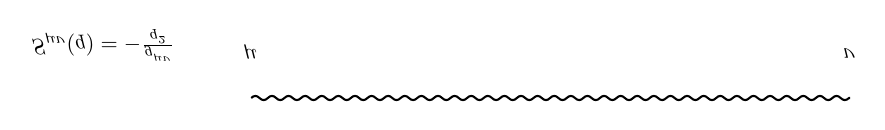
\begin{tikzpicture}[x=0.75pt,y=0.75pt,yscale=-1,xscale=1,scale=0.8, every node/.style={transform shape}]
%uncomment if require: \path (0,69); %set diagram left start at 0, and has height of 69

%Straight Lines [id:da7895899053771676] 
\draw    (154,31) .. controls (155.67,29.33) and (157.33,29.33) .. (159,31) .. controls (160.67,32.67) and (162.33,32.67) .. (164,31) .. controls (165.67,29.33) and (167.33,29.33) .. (169,31) .. controls (170.67,32.67) and (172.33,32.67) .. (174,31) .. controls (175.67,29.33) and (177.33,29.33) .. (179,31) .. controls (180.67,32.67) and (182.33,32.67) .. (184,31) .. controls (185.67,29.33) and (187.33,29.33) .. (189,31) .. controls (190.67,32.67) and (192.33,32.67) .. (194,31) .. controls (195.67,29.33) and (197.33,29.33) .. (199,31) .. controls (200.67,32.67) and (202.33,32.67) .. (204,31) .. controls (205.67,29.33) and (207.33,29.33) .. (209,31) .. controls (210.67,32.67) and (212.33,32.67) .. (214,31) .. controls (215.67,29.33) and (217.33,29.33) .. (219,31) .. controls (220.67,32.67) and (222.33,32.67) .. (224,31) .. controls (225.67,29.33) and (227.33,29.33) .. (229,31) .. controls (230.67,32.67) and (232.33,32.67) .. (234,31) .. controls (235.67,29.33) and (237.33,29.33) .. (239,31) .. controls (240.67,32.67) and (242.33,32.67) .. (244,31) .. controls (245.67,29.33) and (247.33,29.33) .. (249,31) .. controls (250.67,32.67) and (252.33,32.67) .. (254,31) .. controls (255.67,29.33) and (257.33,29.33) .. (259,31) .. controls (260.67,32.67) and (262.33,32.67) .. (264,31) .. controls (265.67,29.33) and (267.33,29.33) .. (269,31) .. controls (270.67,32.67) and (272.33,32.67) .. (274,31) .. controls (275.67,29.33) and (277.33,29.33) .. (279,31) .. controls (280.67,32.67) and (282.33,32.67) .. (284,31) .. controls (285.67,29.33) and (287.33,29.33) .. (289,31) .. controls (290.67,32.67) and (292.33,32.67) .. (294,31) .. controls (295.67,29.33) and (297.33,29.33) .. (299,31) .. controls (300.67,32.67) and (302.33,32.67) .. (304,31) .. controls (305.67,29.33) and (307.33,29.33) .. (309,31) .. controls (310.67,32.67) and (312.33,32.67) .. (314,31) .. controls (315.67,29.33) and (317.33,29.33) .. (319,31) .. controls (320.67,32.67) and (322.33,32.67) .. (324,31) .. controls (325.67,29.33) and (327.33,29.33) .. (329,31) .. controls (330.67,32.67) and (332.33,32.67) .. (334,31) .. controls (335.67,29.33) and (337.33,29.33) .. (339,31) .. controls (340.67,32.67) and (342.33,32.67) .. (344,31) .. controls (345.67,29.33) and (347.33,29.33) .. (349,31) .. controls (350.67,32.67) and (352.33,32.67) .. (354,31) .. controls (355.67,29.33) and (357.33,29.33) .. (359,31) .. controls (360.67,32.67) and (362.33,32.67) .. (364,31) .. controls (365.67,29.33) and (367.33,29.33) .. (369,31) .. controls (370.67,32.67) and (372.33,32.67) .. (374,31) .. controls (375.67,29.33) and (377.33,29.33) .. (379,31) .. controls (380.67,32.67) and (382.33,32.67) .. (384,31) .. controls (385.67,29.33) and (387.33,29.33) .. (389,31) .. controls (390.67,32.67) and (392.33,32.67) .. (394,31) .. controls (395.67,29.33) and (397.33,29.33) .. (399,31) .. controls (400.67,32.67) and (402.33,32.67) .. (404,31) .. controls (405.67,29.33) and (407.33,29.33) .. (409,31) .. controls (410.67,32.67) and (412.33,32.67) .. (414,31) .. controls (415.67,29.33) and (417.33,29.33) .. (419,31) .. controls (420.67,32.67) and (422.33,32.67) .. (424,31) .. controls (425.67,29.33) and (427.33,29.33) .. (429,31) .. controls (430.67,32.67) and (432.33,32.67) .. (434,31) .. controls (435.67,29.33) and (437.33,29.33) .. (439,31) .. controls (440.67,32.67) and (442.33,32.67) .. (444,31) .. controls (445.67,29.33) and (447.33,29.33) .. (449,31) .. controls (450.67,32.67) and (452.33,32.67) .. (454,31) .. controls (455.67,29.33) and (457.33,29.33) .. (459,31) .. controls (460.67,32.67) and (462.33,32.67) .. (464,31) .. controls (465.67,29.33) and (467.33,29.33) .. (469,31) .. controls (470.67,32.67) and (472.33,32.67) .. (474,31) .. controls (475.67,29.33) and (477.33,29.33) .. (479,31) .. controls (480.67,32.67) and (482.33,32.67) .. (484,31) .. controls (485.67,29.33) and (487.33,29.33) .. (489,31) .. controls (490.67,32.67) and (492.33,32.67) .. (494,31) .. controls (495.67,29.33) and (497.33,29.33) .. (499,31) .. controls (500.67,32.67) and (502.33,32.67) .. (504,31) .. controls (505.67,29.33) and (507.33,29.33) .. (509,31) .. controls (510.67,32.67) and (512.33,32.67) .. (514,31) -- (514.71,31) -- (514.71,31) ;

% Text Node
\draw (20,10.4) node [anchor=north west][inner sep=0.75pt]    {$S_{\mu \nu }( q) =-\frac{g^{\mu \nu }}{q^{2}}$};
% Text Node
\draw (148,9.24) node [anchor=north west][inner sep=0.75pt]    {$\mu $};
% Text Node
\draw (509,8.24) node [anchor=north west][inner sep=0.75pt]    {$\nu $};


\end{tikzpicture}

    \end{center}
\end{itemize}

Cuando tenemos que sumar varios diagramas es importante determinar el signo relativo entre ellos. Para ello debemos ver si la ordenación de los espinores en las amplitudes es la misma o no. Así por ejemplo, dos amplitudes con espinores $\bar{u} u \bar{v} v$ y $\bar{v} u \bar{u} v$ tendrán signos opuestos puesto que requieren intercambiar el orden de operadores de creación o destrucción fermiónicos.

Basta con coger el orden de las partículas calculadas en la amplitud de dispersión y hacer permutaciones de 2 a 2 partículas cambiendo el signdo en cada una de las permutaciones para ver el signo relativo de cada canal

\begin{example}[Ejemplo de signos relativos]
  Dada la siguiente amplitud de dispersión
  \begin{DispWithArrows}[format=c, displaystyle]
    \frac{e^2}{q^2} [\overline{u}_3\gamma^\mu u_1][\overline{u}_4\gamma^\nu u_2]
  \end{DispWithArrows}

  Vemos que se encuentra en el orden 
  \begin{DispWithArrows}[format=c, displaystyle]
  3142 \Arrow{Un cambio} \\
  -1342 \Arrow{Otro cambio} \\
  1324 \Arrow{Cambio final} \\
  -1234
  \end{DispWithArrows}
  Como vemos el signo de esta amplitud de dispersión será negativo. 
\end{example}
\subsection{Alguna fórmulas útiles}
\begin{equation}
  \begin{array}{ll}
  g_\mu^\mu=4=\delta_\mu^\mu & \gamma^0=\gamma^{0^ \dagger} \\
  \left\{\gamma^\mu, \gamma^\nu\right\}=2 g^{\mu \nu} & \gamma^i=-\gamma^{i ^\dagger} \\
  \gamma_\nu \gamma^\mu \gamma^\nu=-2 \gamma^\mu & \left(\gamma^0\right)^2=1 \\
  \gamma_{\mu}=g_{\mu\nu} \gamma^\nu &\gamma^{\mu^\dagger}=\gamma^\sigma \gamma^\mu \gamma^\sigma \\
  \gamma^\rho \gamma^\mu \gamma^\nu \gamma_\rho=4 g^{\mu \nu} & \\
  \gamma^\mu \gamma^\nu \gamma^\rho \gamma^\sigma \gamma_\mu=-2 \gamma^\sigma \gamma^\rho \gamma^\nu
  \end{array}
  \end{equation}

  $\gamma ^5$ no aparece en la electrodínamica cuántica, pero si aparece cuando hay interacción de la fuerza débil. Algunas propiedades són:

  \begin{equation}
    \begin{aligned}
    & \gamma^5=i \gamma^0 \gamma^1 \gamma^2 \gamma^3 \quad\left(\gamma^5\right)^2=\mathbb{I}\quad  \gamma^5=\gamma^{5^\dagger} \quad\left\{\gamma^5, \gamma^\nu\right\}=0 \\
    & P_L=1 / 2\left(1-\gamma^5\right) \quad P_R=1 / 2\left(1+\gamma^s\right) \\
    & P_L^2=P_L \quad P_R^2=P_R \quad P_L+R_R=\mathbb{I}
    \end{aligned}
    \end{equation}

    Algunas propiedades sobre traza son:
    
    \begin{equation}
      \begin{aligned}
      \operatorname{Tr}\left(\gamma_{\mu\nu}\right)=0\Leftrightarrow\nu\text{ impar} \quad& \quad\operatorname{Tr}\left(\gamma^5\right)=0 \\
      \operatorname{Tr}\left(\gamma_\mu\gamma_\nu\right)=4g_{\mu\nu}\quad& \quad \operatorname{Tr}\left(\gamma^\mu \gamma^5\right)=0 \\
      \operatorname{Tr}\left(\gamma_\mu\gamma_\nu\gamma_{\sigma\rho}\right)=4\left(g_{\mu\nu}g_{\rho\sigma}-g_{\mu\rho}g_{\nu\sigma}+g_{\mu\sigma}g_{\nu\rho}\right)\quad& \quad \operatorname{Tr}\left(\gamma^\mu \gamma^\nu \gamma^5\right)=0 \\
      \quad& \quad \operatorname{Tr}\left(\gamma^\mu \gamma^\nu \gamma^\sigma \gamma^5\right)=0 \\
      \quad& \quad \operatorname{Tr}\left(\gamma^\mu \gamma^\nu \gamma^\sigma \gamma^\rho \gamma^5\right)=4i\epsilon^{\mu\nu\sigma\rho}
      \end{aligned}
      \end{equation}
      \pagelayout{wide}
\section{Procesos en electrodinámica cuántica}
\subsection{Dispersión Möller}
\begin{figure}
  \centering
  \includegraphics{Moller.png}
  \caption{Diagramás de Feymann de la dispersión Möller}
\end{figure}
\subsubsection{Canal t}
A partir del diagrama, podemos escribir el elemento de matriz:

\begin{equation}
\mathcal{M}_t = (ei\overline{u}_3\gamma^\mu u_1) \frac{ig_{\mu\nu}}{q^2} (ei\overline{v}_4\gamma^\nu u_2) = \frac{e^2}{q^2} [\overline{u}_3\gamma^\mu u_1][\overline{u}_4\gamma^\nu u_2],
\end{equation}

donde el momento del propagador $ q = p_1 - p_3 = \sqrt{t} $. El módulo al cuadrado es

\begin{equation}
\begin{aligned}
|\mathcal{M}_t|^2 &= \frac{e^4}{t^2} [\overline{u}_3\gamma^\mu u_1][\overline{u}_4\gamma^\nu u_2]^* [\overline{u}_3\gamma^\mu u_1]^*[\overline{u}_4\gamma^\nu u_2] \\
&= \frac{e^4}{t^2} [\overline{u}_3\gamma^\mu u_1][\overline{u}_1 \gamma^\rho u_3] [\overline{u}_2 \gamma^\sigma v_4] [\overline{u}_4\gamma^\nu u_2] \\
&= \frac{e^4}{t^2} [\overline{u}_3\gamma^\mu u_1][\overline{u}_1 \gamma^\rho u_3] [\overline{u}_4\gamma^\nu u_1^a][\overline{u}_2 \gamma^\sigma v_4],
\end{aligned}
\end{equation}

donde hemos utilizado la identidad:

\begin{equation}
[\overline{u} \gamma^\rho v]^* = [\overline{u} \gamma^\rho v]^\dagger = v^\dagger \gamma^0 \gamma^\rho \gamma^0 u = v^\dagger (\gamma^0)^2 \gamma^\rho \gamma^0 u = \overline{v} \gamma^\rho u.
\end{equation}
lo cual es válido para espinores $ u $ y $ v $. Dado que las cantidades entre corchetes son números $ C $, podemos tomar sus trazas sin repercusiones:

\begin{equation}
  \begin{aligned}
    |\mathcal{M}_t|^2 = \frac{e^4}{t^2} \text{Tr}[\overline{u}_3\gamma^\nu u_1 \overline{u}_1 \gamma^\nu u_3] \text{Tr}[\overline{u}_2 \gamma^\mu u_4 \overline{u}_4 \gamma^\mu u_2] \\ = \frac{e^4}{t^2} \text{Tr}[u_1 \overline{u}_1 \gamma^\nu u_3 \overline{u}_3 \gamma^\mu] \text{Tr}[u_2 \overline{u}_2 \gamma^\mu u_4 \overline{u}_4 \gamma^\nu].
  \end{aligned}

\end{equation}

Ahora debemos promediar sobre los espines iniciales y sumar sobre los espines finales:

\begin{equation}
|\overline{\mathcal{M}_t}|^2 = \frac{e^4}{4t^2} \text{Tr} \left[ \sum_s u_1^s \overline{u}_1^s \gamma^\nu \sum_{s'} u_3^{s'} \overline{u}_3^{s'} \gamma^\mu \right] \text{Tr} \left[ \sum_r v_2^r \overline{v}_2^r \gamma^\mu \sum_{r'} v_4^{r'} \overline{v}_4^{r'} \gamma^\nu \right],
\end{equation}

usamos las relaciones de completitud para los espinores de Dirac:

\begin{equation}
|\overline{\mathcal{M}_t}|^2 = \frac{e^4}{4t^2} \text{Tr} \left[ (\not{p}_1 - m_e) \gamma^\nu (\not{p}_3 - m_e) \gamma^\mu \right] \text{Tr} \left[ (\not{p}_2 - m_e) \gamma^\mu (\not{p}_4 - m_e) \gamma^\nu \right],
\end{equation}

aquí notaremos que cualquier término que sea lineal en la masa del electrón contendrá un número impar de matrices de Dirac dentro de una traza, la cual se evalúa a cero. Por lo tanto:

\begin{equation}
|\mathcal{M}_t|^2 = \frac{e^4}{4t^2} \left\{ \text{Tr} \left[ \not{p}_1 \not{p}_3 \gamma^\nu \not{p}_3 \gamma^\mu \right] + m_e^2 \, \text{Tr} \left[ \gamma^\nu \gamma^\mu \right] \right\} \left\{ \text{Tr} \left[ \not{p}_2 \not{p}_4 \gamma^\mu \not{p}_4 \gamma^\nu \right] + m_e^2 \, \text{Tr} \left[ \gamma^\mu \gamma^\nu \right] \right\},
\end{equation}

usando las identidades de traza de las matrices de Dirac (Peskin Apéndice 3) esto es

\begin{equation}
\begin{aligned}
  |\overline{\mathcal{M}_t}|^2 = \frac{e^4}{4t^2} \left\{ \not{p}_1 \not{p}_3 \, \text{Tr} \left[ \gamma^\nu \gamma^\mu \right] + 4 g_{\mu \nu} m_e^2 \right\} \left\{  p_{2\alpha} p_{4\beta} \, \text{Tr} \left[ \gamma^\mu \gamma^\nu \right]\right. \\
  \left. + 4 g_{\mu \nu} m_e^2 \right\},
\end{aligned}
\end{equation}

las trazas restantes son

\begin{DispWithArrows}[format=c, displaystyle]
  
    p_{1\alpha} p_{3\beta} \, \text{Tr} \left[ \gamma^\alpha \gamma^\beta \gamma^\nu \gamma^\mu \right] = 4 p_{1 \alpha} p_{3 \beta} \left( g^{\alpha \beta} g^{\nu \mu} - g^{\alpha \nu} g^{\beta \mu} + g^{\alpha \mu} g^{\beta \nu} \right) \\
    
    
    = 4 (p_{1\mu} p_{3\nu} - (p_1 \cdot p_3) g_{\mu\nu} + p_{1\nu} p_{3\mu}) \\
    
    
    = 4 p_{2\alpha} p_{4\beta} \left( g^{\alpha \beta} g^{\mu \nu} - g^{\alpha \mu} g^{\beta \nu} + g^{\alpha \nu} g^{\beta \mu} \right) \\
    
    
    = 4 (p_{2\mu} p_{4\nu} - (p_2 \cdot p_4) g_{\mu\nu} + p_{2\nu} p_{4\mu}) \\
\end{DispWithArrows}

Ahora debemos realizar la multiplicación en la expansión de las matrices. El primer término es la contracción de las dos trazas anteriores, así que usando la notación (1+2+3)(A+B+C), los términos son


las cuales debemos sumar (incluyendo un factor global de $4^2$), observa que el factor de 4 en 2B proviene de $g^{\mu\nu}g_{\mu\nu} = 4$. Notemos las relaciones:

$ 1A = 3C \quad 1C = 3A \quad 2B + 1B + 2A + 2C + 3B = 0, $

así que su suma es

\begin{equation}
4^2 \left[ 2(p_2 \cdot p_1)(p_4 \cdot p_3) + 2(p_4 \cdot p_1)(p_2 \cdot p_3) \right].
\end{equation}

El segundo término (en el elemento de matriz) es la contracción de los dos términos de masa:

\begin{equation}
4^2 g_{\mu\nu} g^{\mu\nu} m_e^4 = 4^2 [4m_e^4].
\end{equation}

Los dos términos restantes son los "términos cruzados":

\begin{DispWithArrows}[format=ll, displaystyle]
  
    4 (p_{1\mu} p_{3\beta} - (p_1 \cdot p_3) g_{\mu \nu} + p_{1\nu} p_{3\mu})(4g_{\mu \nu} m_e^2) &= 4^2 \left[ m_e^2 (p_1 \cdot p_3 - 4p_1 \cdot p_3 + p_1 \cdot p_3) \right] \\
    
   & = 4^2 \left[ -2m_e^2 p_1 \cdot p_3 \right],
    
\end{DispWithArrows}

y

\begin{DispWithArrows}[format=ll, displaystyle]
  
  4 (p_2^\beta p_4^\alpha - (p_2 \cdot p_4) g_{\mu \nu} + p_4^\beta p_2^\alpha)(4g_{\mu \nu} m_e^2) &= 4^2 \left[ m_e^2 (p_2 \cdot p_4 - 4(p_2 \cdot p_4) + p_2 \cdot p_4) \right] \\
  
 & = 4^2 \left[ -2m_e^2 p_2 \cdot p_4 \right].,
  
\end{DispWithArrows}


Reuniendo estos términos, el elemento de matriz es

\begin{equation}
\begin{aligned}
  |\overline{\mathcal{M}_t}|^2 = \frac{e^4}{t^2} \left\{ 2(p_2 \cdot p_1)(p_4 \cdot p_3) + 2(p_4 \cdot p_1)(p_2 \cdot p_3) + 4m_e^4 \right.\\
\left.- 2m_e^2(p_1 \cdot p_3) - 2m_e^2(p_2 \cdot p_4) \right\}.
\end{aligned}
\end{equation}

Nuevamente utilizaremos nuestros invariantes de Mandelstam, observando (en el caso masivo)

\begin{equation}
-2p_1 \cdot p_2 = s - 2m_e^2 = 2ps \cdot p_4,
\end{equation}

\begin{equation}
-2p_1 \cdot p_3 = t - 2m_e^2 = -2p_2 \cdot p_4,
\end{equation}

\begin{equation}
-2p_1 \cdot p_4 = u - 2m_e^2 = -2p_2 \cdot p_3.
\end{equation}

Con estos, el cuadrado del elemento de matriz es

\begin{equation}
|\mathcal{M}_t|^2 = \frac{e^4}{t^2} \left[ (2(p_1 \cdot p_2)(p_4 \cdot p_3) + (2(p_4 \cdot p_1)(p_2 \cdot p_3) + 8m_e^4 - 4m_e^2(p_1 \cdot p_3) - 4m_e^2(p_2 \cdot p_4) \right]
\end{equation}

\begin{equation}
= \frac{e^4}{t^2} \left[ (s - t - m_e^2)^2 + (u - t - m_e^2)^2 + 8m_e^4 + 2m_e^2(t - 2m_e^2) + 2m_e^2(t - 2m_e^2) \right]
\end{equation}

\begin{equation}
= \frac{e^4}{t^2} \left[ s^2 + u^2 + 2sm_e^2 + 2um_e^2 + 4m_e^4 + 2m_e^2(t - 2m_e^2) \right]
\end{equation}

\begin{equation}
= \frac{e^4}{t^2} \left[ s^2 + u^2 + 2sm_e^2 + 2um_e^2 + 4m_e^4 + 4m_e^2t - 8m_e^4 \right]
\end{equation}

\begin{equation}
= \frac{e^4}{t^2} \left[ s^2 + u^2 - 2m_e^2s - 2m_e^2u + 4m_e^2t - 8m_e^4 \right].
\end{equation}

Recuperamos, en el límite ultrarrelativista (i.e., electrón sin masa):

\begin{equation}
|\overline{\mathcal{M}_t}|^2 = 2e^4 \frac{s^2 + u^2}{t^2}.
\end{equation}

\subsubsection{Canal u}

A partir del diagrama, podemos escribir el elemento de matriz:

\begin{equation}
\mathcal{M}_u = (ei\overline{u}_3\gamma^\nu u_1) \frac{ig_{\nu\rho}}{q^2} (ei\overline{u}_4\gamma^\rho u_2) = \frac{e^2}{q^2} [\overline{u}_3\gamma^\nu u_1][\overline{u}_4\gamma^\rho u_2],
\end{equation}

el análisis que sigue se abreviará porque el proceso es casi idéntico al canal t. El cuadrado del módulo del elemento de matriz es

\begin{equation}
|\mathcal{M}_u|^2 = \left( \frac{e^2}{q^2} \right)^2 \left[ [\overline{u}_3\gamma^\nu u_1][\overline{u}_4\gamma^\rho u_2] \right]\left[[\overline{u}_3\gamma_\nu u_1][\overline{u}_2\gamma_\rho u_4]\right]
\end{equation}

\begin{equation}
= \frac{e^4}{q^4} \left[ [\overline{u}_3\gamma^\nu u_1][\overline{u}_4\gamma^\rho u_2]^*[ [\overline{u}_3\gamma_\nu u_1]^*[\overline{u}_2\gamma_\rho u_4] \right]
\end{equation}

\begin{equation}
= \frac{e^4}{q^4} \text{Tr}[u_1\overline{u}_1\gamma^\nu u_4\overline{u}_4\gamma^\rho] \text{Tr}[u_3\overline{u}_3\gamma_\nu u_2\overline{u}_2\gamma_\rho],
\end{equation}

ahora sumamos y promediamos sobre los espines finales e iniciales, y usamos las relaciones de completitud para los espinores de Dirac:

\begin{equation}
|\overline{\mathcal{M}_u}|^2 = \frac{e^4}{4u^2} \text{Tr}[(\not{p}_1 + m)\gamma^\nu (\not{p}_4 + m)\gamma^\rho] \text{Tr}[(\not{p}_2 + m)\gamma^\rho (\not{p}_3 + m)\gamma^\nu]
\end{equation}

\begin{equation}
= \frac{e^4}{4u^2} \left\{ \text{Tr} \left[ \not{p}_1 \not{p}_4 \gamma^\nu \not{p}_4 \gamma^\rho \right] + m^2 \text{Tr}[\gamma^\nu\gamma^\rho] \right\} \left\{ \text{Tr} \left[ \not{p}_2 \not{p}_3 \gamma^\rho \not{p}_3 \gamma^\nu \right] + m^2 \text{Tr}[\gamma^\rho\gamma^\nu] \right\}
\end{equation}

\begin{equation}
= \frac{e^4}{4u^2} \left\{ p_{1\alpha}p_{4\beta} \text{Tr}[\gamma^\alpha\gamma^\beta\gamma^\nu\gamma^\rho] + 4g_{\nu\rho}m^2 \right\} \left\{ p_{2\alpha}p_{3\beta} \text{Tr}[\gamma^\rho\gamma^\nu\gamma^\beta\gamma^\alpha] + 4g_{\rho\nu}m^2 \right\},
\end{equation}

las trazas restantes son

\begin{equation}
p_1^\alpha p_4^\beta \text{Tr}[\gamma_\alpha\gamma_\beta\gamma_\nu\gamma_\rho] = 4p_1^\alpha p_4^\beta (g_{\alpha\nu}g_{\beta\rho} - g_{\alpha\beta}g_{\nu\rho} + g_{\alpha\rho}g_{\beta\nu})
\end{equation}

\begin{equation}
= 4(p_1\cdot p_4)(p_2\cdot p_3) - 4(p_1\cdot p_3)(p_2\cdot p_4),
\end{equation}

\begin{equation}
p_{2\alpha}p_{3\beta} \text{Tr}[\gamma_\rho\gamma_\nu\gamma^\beta\gamma^\alpha] = 4p_{2\alpha}p_{3\beta}\left(g_{\rho\beta}g_{\nu\alpha} - g_{\rho\nu}g_{\beta\alpha} + g_{\rho\alpha}g_{\nu\beta}\right)
\end{equation}

\begin{equation}
= 4(p_2\cdot p_3)(g_{\rho\nu} - (p_2\cdot p_4)) + 4(p_4\cdot p_3),
\end{equation}

que se contraen para dar

\begin{equation}
4^2[2(p_2\cdot p_1)(p_4\cdot p_3) + 2(p_3\cdot p_1)(p_2\cdot p_4)].
\end{equation}

El producto de términos de masa es

\begin{equation}
4^2[4m^4],
\end{equation}

y los términos cruzados son

\begin{equation}
4(p_{1\mu}p_{4\nu} - (p_1\cdot p_4)g_{\mu\nu} + p_{1\nu}p_{4\mu})4m_e^2g_{\mu\nu} = 4^2[-2m_e^2(p_1\cdot p_4)]
\end{equation}

\begin{equation}
4(p_2^\alpha p_3^\beta - (p_2\cdot p_3)g_{\rho\nu} + p_3^\alpha p_2^\beta)4m_e^2g_{\rho\nu} = 4^2[-2m_e^2(p_2\cdot p_3)],
\end{equation}

así que el cuadrado del elemento de matriz es

\begin{equation}
|\overline{\mathcal{M}_u}|^2 = \frac{e^4}{u^2} \left[ 2(p_2 \cdot p_1)(p_4 \cdot p_3) + 2(p_3 \cdot p_1)(p_2 \cdot p_4) + 4m_e^4 - 2m_e^2(p_1 \cdot p_4) - 2m_e^2(p_2 \cdot p_3) \right].
\end{equation}
Escribiendo esto en términos de invariantes de Mandelstam, tenemos

\begin{equation}
|\overline{\mathcal{M}_u}|^2 = \frac{e^4}{u^2} \left\{ 2(p_2 \cdot p_1)(p_3 \cdot p_4) + (-2)(p_3 \cdot p_1)(-2)(p_2 \cdot p_4) + 8m_e^4 - 4m_e^2(p_1 \cdot p_4) - 4m_e^2(p_2 \cdot p_3) \right\},
\end{equation}

\begin{equation}
= \frac{e^4}{u^2} \left\{ [(s - m_e^2)^2 + (t - m_e^2)^2 + 8m_e^4 + 2m_e^2(u - m_e^2) + 2m_e^2(u - m_e^2)] \right\},
\end{equation}

\begin{equation}
|\overline{\mathcal{M}_u}|^2 = \frac{e^4}{u^2} \left[ s^2 + t^2 + 2m_e^2(2u - s - t) + 4m_e^4 \right].
\end{equation}

Recuperamos, en el límite ultrarrelativista (i.e., electrón sin masa):

\begin{equation}
|\overline{\mathcal{M}_u}|^2 = 2e^4 \frac{s^2 + t^2}{u^2}.
\end{equation}

Es interesante notar que podríamos haber encontrado este resultado si hubiéramos hecho las sustituciones $ p_3 \to p_4 $ y $ p_4 \to p_3 $ (nótese que no necesitamos considerar un cambio de signo, ya que no estamos tratando con antipartículas), por lo que los invariantes de Mandelstam se convierten en

\begin{equation}
s = (p_1 + p_2)^2 \rightarrow (p_1 + p_2)^2 = s,
\end{equation}

\begin{equation}
t = (p_3 - p_1)^2 \rightarrow (p_4 - p_1)^2 = u,
\end{equation}

\begin{equation}
u = (p_4 - p_1)^2 \rightarrow (p_3 - p_1)^2 = t.
\end{equation}

\subsubsection{Términos cruzados}
El primer término cruzado es

\begin{equation}
\mathcal{M}_t \mathcal{M}_u^* = \frac{1}{4} \sum_{\text{spins}} \left[ \frac{e^2}{t} [\bar{u}_3 \gamma^\mu u_1] [\bar{u}_4 \gamma_\mu u_2] \right] \left[ \frac{e^2}{u^2} [\bar{u}_4 \gamma^\nu u_1] [\bar{u}_3 \gamma_\nu u_2] \right]
\end{equation}

\begin{equation}
= \frac{e^4}{4tu} \sum_{\text{spins}} [\bar{u}_3 \gamma^\nu u_1] [\bar{u}_4 \gamma_\nu u_2] [\bar{u}_4 \gamma^\mu u_2] [\bar{u}_3 \gamma_\mu u_3]
\end{equation}

\begin{equation}
= \frac{e^4}{4tu} \sum_{\text{spins}} \text{Tr}[\gamma_\nu u_1 \bar{u}_1 \gamma^\mu u_2 \bar{u}_2 \gamma_\mu u_3 \bar{u}_3]
\end{equation}

\begin{equation}
= \frac{e^4}{4tu} \text{Tr}[(\slashed{q}_3 + m) \gamma_\nu (\slashed{p}_4 + m)\gamma^\mu (\slashed{p}_2 + m)\gamma^\nu (\slashed{p}_3 + m)]
\end{equation}

\begin{equation}
= \frac{e^4}{4tu} g_{\mu \rho} g_{\nu \sigma} \text{Tr}[\gamma^\rho (\slashed{p}_4 + m) \gamma^\mu (\slashed{p}_2 + m) \gamma^\sigma (\slashed{p}_3 + m)]
\end{equation}

\begin{equation}
= \frac{e^4}{4tu} g_{\mu \rho} g_{\nu \sigma} \text{Tr}[\gamma^\rho \slashed{p}_4 \gamma^\mu \slashed{p}_2 \gamma^\sigma \slashed{p}_3 ]
\end{equation}

Por el bien de los cálculos, pongamos esto en una forma diferente, usando $ p_1 \to p, \, p_2 \to k,\, p_3 \to p', \, p_4 \to k' $, entonces podemos escribir el término cruzado como

\begin{equation}
\mathcal{M}_t \mathcal{M}_u^* = \frac{e^4}{4st} g_{\mu \alpha} g_{\nu \beta} \text{Tr}[\gamma^\alpha \slashed{k}' \gamma^\mu \slashed{k} \gamma^\beta \slashed{p}'] = \frac{e^4}{4st} g_{\mu \alpha} g_{\nu \beta} \text{Tr}[\gamma^\alpha \slashed{k}' \gamma^\nu \slashed{p} \gamma^\mu \slashed{p}']
\end{equation}

ahora renombramos nuestros índices (intercambiando $\beta$ y $\mu$):

\begin{equation}
\mathcal{M}_t \mathcal{M}_u^* = \frac{e^4}{4tu} g_{\alpha \beta} g_{\mu \nu} \text{Tr}[\gamma^\alpha \gamma^\rho \gamma^\beta \slashed{k}' \slashed{p} \gamma^\nu]
\end{equation}

Nota las siguientes relaciones que se pueden encontrar en el Apéndice A.4 de Schwartz \textit{Quantum Field Theory and the Standard Model}:

\begin{equation}
\gamma^\nu \gamma^\nu = 4
\end{equation}

\begin{equation}
\gamma^\nu \gamma^\mu \gamma^\nu = -2\gamma^\mu
\end{equation}

\begin{equation}
\gamma^\nu \gamma^\mu \gamma^\rho \gamma^\nu = 4g^{\mu \rho}
\end{equation}

\begin{equation}
\gamma^\nu \gamma^\mu \gamma^\rho \gamma^\sigma \gamma^\nu = -2\gamma^\sigma \gamma^\rho \gamma^\mu
\end{equation}

y nota que la cuarta vale para cualquier cantidad impar de matrices gamma entre dos matrices gamma contraídas. Por lo tanto:

\begin{equation}
\mathcal{M}_t \mathcal{M}_u^* = \frac{e^4}{4tu} g_{\alpha \beta} \text{Tr}[\gamma^\alpha \gamma^\rho \gamma^\beta \slashed{k}' \slashed{p} \slashed{p}'] = \frac{e^4}{2tu} g_{\alpha \beta} \text{Tr}[\slashed{k} \gamma^\nu \slashed{p} \gamma^\alpha \gamma^\beta \gamma^\rho]
\end{equation}

\begin{equation}
= \frac{e^4}{2tu} e^2 (p \cdot k')\text{Tr}[\slashed{p} \slashed{k} \gamma^\nu] = e^4 \left( \frac{p_2 \cdot p_4}{p\cdot k'} \right) \text{Tr}[\slashed{p} \cdot \slashed{k}]
\end{equation}

Ahora en términos de los momentos definidos originalmente:

\begin{equation}
\mathcal{M}_t \mathcal{M}_u^* = \frac{-e^8}{stu} (p_1, p_2) (p_3, p_4)
\end{equation}

En términos de los invariantes de Mandelstam esto es

\begin{equation}
\mathcal{M}_t \mathcal{M}_u^* = -8 \frac{e^4}{tu} \left( \frac{s}{2} \right) \left( \frac{s}{2} \right) = -2e^4 \frac{s^2}{tu}.
\end{equation}

En lugar de calcular el otro término cruzado, afirmaré

\begin{equation}
2\text{Re}\{\mathcal{M}_t \mathcal{M}_u^*\} = \mathcal{M}_t \mathcal{M}_u^* + \mathcal{M}_t^* \mathcal{M}_u = 2\text{Re}\{\mathcal{M}_t^* \mathcal{M}_u\},
\end{equation}
así que

\begin{equation}
\mathcal{M}_t \mathcal{M}_u^* + \mathcal{M}_t^* \mathcal{M}_u = -4e^4 \frac{s^2}{tu}.
\end{equation}

\subsubsection{Sección eficaz diferencial}
Para un estado final de dos cuerpos, la sección transversal diferencial está dada por (Peskin eq. 5.12)

\begin{equation}
\frac{d\sigma}{d\Omega} = \frac{1}{2E_{\text{cm}}^2} \frac{|\mathbf{k}|}{16\pi^2 E_{\text{cm}}} |\mathcal{M}|^2.
\end{equation}

En el límite sin masa, en el marco del centro de masa, la sección transversal diferencial se simplifica a

\begin{equation}
\frac{d\sigma}{d\Omega} = \frac{1}{2E_{\text{cm}}} \frac{E_{\text{cm}}/2}{16\pi^2 E_{\text{cm}}} |\mathcal{M}|^2 = \frac{1}{4E_{\text{cm}}} \frac{1}{(4\pi)^2} |\mathcal{M}|^2.
\end{equation}

Usando los elementos de matriz de las secciones sin masa, tenemos

\begin{equation}
\frac{d\sigma}{d\Omega}_t = \frac{1}{4E_{\text{cm}}^2 (4\pi)^2 t^2} e^4 = \left( \frac{\alpha^2}{2s} \right) \frac{s^2 + u^2}{t^2},
\end{equation}

\begin{equation}
\frac{d\sigma}{d\Omega}_u = \frac{1}{4E_{\text{cm}}^2 (4\pi)^2 u^2} e^4 = \left( \frac{\alpha^2}{2s} \right) \frac{s^2 + t^2}{u^2},
\end{equation}

\begin{equation}
\frac{d\sigma}{d\Omega}_{\text{int}} = \frac{1}{4E_{\text{cm}}^2 (4\pi)^2} \frac{e^4 s^2}{tu} = \left( \frac{\alpha^2}{2s} \right) \left( 2 - \frac{s^2}{tu} \right).
\end{equation}

Ahora necesitamos calcular la suma de las secciones transversales diferenciales, pero primero debemos determinar su signo. Como hay fermiones idénticos en el estado final, tenemos que:

\begin{equation}
\mathcal{M} = \mathcal{M}_t - \mathcal{M}_u \quad \Rightarrow \quad |\mathcal{M}|^2 = |\mathcal{M}_t|^2 + |\mathcal{M}_u|^2 - \mathcal{M}_t \mathcal{M}_u^* - \mathcal{M}_t^* \mathcal{M}_u,
\end{equation}

ya que bajo el intercambio de partículas, los sistemas fermiónicos son impares. Entonces

\begin{equation}
\frac{d\sigma}{d\Omega} = \frac{d\sigma}{d\Omega}_t + \frac{d\sigma}{d\Omega}_u + \frac{d\sigma}{d\Omega}_{\text{int}}.
\end{equation}

poniendo nuestros resultados:

\begin{equation}
\frac{d\sigma}{d\Omega} = \frac{\alpha^2}{2s} \left[ \frac{s^2 + u^2}{t^2} + \frac{s^2 + t^2}{u^2} - 2 \left( \frac{t}{u} \right)^2 - 2 \left( \frac{u}{t} \right)^2 \right],
\end{equation}

que se puede escribir como

\begin{equation}
\frac{d\sigma}{d\Omega} = \frac{\alpha^2}{2s} \left( \left( \frac{u}{t} \right)^2 + \left( \frac{t}{u} \right)^2 + \frac{1}{s^2} \right) .
\end{equation}

Si integramos sobre el azimut, adquirimos un factor de $2\pi$, por lo tanto

\begin{equation}
\frac{d\sigma}{d\cos\theta} = \frac{\pi \alpha^2}{s} \left( \left( \frac{u}{t} \right)^2 + \left( \frac{t}{u} \right)^2 + 2 s + \left( \frac{1}{u} \right)^2 + \frac{1}{t^2} \right).
\end{equation}

Investigamos la dependencia angular de la sección transversal diferencial. En el marco del centro de masa, tenemos

$$\begin{aligned}
  p_1 &= (E_{\text{cm}}/2, \mathbf{p}), \\
  p_2 &= (E_{\text{cm}}/2, -\mathbf{p}), \\
  p_3 &= (E_{\text{cm}}/2, \mathbf{k}), \\
  p_4 &= (E_{\text{cm}}/2, -\mathbf{k}).
  \end{aligned}$$

  donde $|\mathbf{p}| = |\mathbf{k}| = E_{\text{cm}}/2$. Usando esto, los invariantes de Mandelstam se pueden escribir como

\begin{equation}
s = 2p_1 \cdot p_2 = E_{\text{cm}}^2
\end{equation}

\begin{equation}
t = -2p_1 \cdot p_3 = -2(p_1^0 p_3^0 - (\mathbf{p} \cdot \mathbf{k}))
= -\frac{E_{\text{cm}}^2}{4} (1 - \cos \theta)
\end{equation}

\begin{equation}
u = -2p_1 \cdot p_4 = -2(p_1^0 p_4^0 - (\mathbf{p} \cdot -\mathbf{k}))
= -\frac{E_{\text{cm}}^2}{4} (1 + \cos \theta)
\end{equation}

Insertando esto en la expresión de la sección transversal diferencial obtenemos

\begin{equation}
\frac{d\sigma}{d\cos \theta} = \frac{\pi \alpha^2}{s} \left[ \left( \frac{-E_{\text{cm}}^2/4}{1 - \cos \theta} \right)^2 + \left( \frac{-E_{\text{cm}}^2/4}{1 + \cos \theta} \right)^2
+ E_{\text{cm}}^4 \left( \frac{1}{-E_{\text{cm}}^2/4 (1 - \cos \theta)} + \frac{1}{-E_{\text{cm}}^2/4 (1 + \cos \theta)} \right)^2 \right]
\end{equation}

la simplificación da como resultado

\begin{equation}
\frac{d\sigma}{d\cos \theta} = \frac{\pi \alpha^2}{s} \left[ \left( \frac{1 + \cos \theta}{1 - \cos \theta}\right)^2 + \left( \frac{1 - \cos \theta}{1 + \cos \theta} \right)^2 + 4 \left( \frac{1}{1 - \cos \theta} + \frac{1}{1 + \cos \theta} \right)^2 \right]
\end{equation}

dejando que nuestro viejo amigo \textsl{MATHEMATICA} maneje el álgebra, obtenemos

\begin{equation}
\frac{d\sigma}{dx} = \frac{\pi \alpha^2}{E_{\text{cm}}^2} \left[ \frac{2 (x^2 + 3)}{(x^2 - 1)^2} \right],
\end{equation}

donde $x = \cos \theta$. Podemos integrar la dependencia angular para ver la dependencia en la energía del centro de masa:

\begin{equation}
\sigma = \int \frac{\pi \alpha^2}{E_{\text{cm}}^2} \left[ \frac{2 (x^2 + 3)}{(x^2 - 1)^2} \right] \, dx = \frac{\pi \alpha^2}{E_{\text{cm}}^2} \left[ x - \frac{8x}{x^2 - 1} \right],
\end{equation}

que diverge en $\pm 1$. Si limitamos la medición a partículas con un ángulo de dispersión mayor que 10°, podemos evaluar la integral numéricamente:

\begin{equation}
\sigma = \int_{\cos(170^\circ)}^{\cos(10^\circ)} \frac{\pi \alpha^2}{E_{\text{cm}}^2} \frac{2 (x^2 + 3)}{(x^2 - 1)^2} \, dx = 1049.05 \frac{\pi \alpha^2}{E_{\text{cm}}^2},
\end{equation}

tener en cuenta que las unidades son GeV$^{-2}$, por lo que tomamos un factor de:

\begin{equation}
\sigma = 1049.05 \frac{0.3894 \, \text{mb}}{1 \, \text{GeV}^{-2}} = \frac{0.06837}{(E_{\text{cm}}/\text{GeV})^2} \, \text{mb}.
\end{equation}

Ahora necesitamos incluir un factor de 1/2 debido a las partículas idénticas en el estado final$^\dagger$, así que

\begin{equation}
\sigma = \frac{0.0342}{(E_{\text{cm}}/\text{GeV})^2} \, \text{mb}.
\end{equation}

Por ejemplo, en haces de electrones colisionando, cada uno con un momento de 4000 GeV (para un \textsl{center-of-mass} de energía de 8000 GeV), la sección transversal total (para la dispersión mayor de 10°) es $\sigma = 5.342 \times 10^{-10}$ mb o 0.534 pb.


\subsection{Dispersión Blhaba}
Hay dos diagramas de Feynman que contribuyen en el proceso:
\begin{figure}
  \centering
  \includegraphics{Bhabha.png}
  \caption{Diagramás de Feymann de la dispersión Bhabha}
\end{figure}
Con amplitudes que denotamos como $ A^{(1)} $ y $ A^{(2)} $ respectivamente. Usando las reglas de Feynman, podemos traducir los diagramas de Feynman en amplitudes:

\begin{equation}
iA^{(1)} = \bar{u}(k')(-ie\gamma^\mu)u(p) \left( \frac{-ig_{\mu\nu}}{q^2} \right) \bar{v}(p')(-ie\gamma^\nu)v(k')
\end{equation}

donde $ q = p - p' = k' - k $.

\begin{equation}
iA^{(2)} = \bar{u}(k')(-ie\gamma^\nu)u(p) \left( \frac{-ig_{\mu\nu}}{q^2} \right) \bar{v}(p')(-ie\gamma^\mu)v(k')
\end{equation}

La amplitud total del proceso es la suma de estos dos:

\begin{equation}
\mathcal{A} = iA^{(1)} + iA^{(2)} 
\end{equation}

Para simplificar las expresiones, introduciremos las variables de Mandelstam:

\begin{equation}
t = (p_1 + p_2)^2 = (p'_1 + p'_2)^2
\end{equation}

\begin{equation}
s = (p_1 - p'_1)^2 = (p_2 - p'_2)^2
\end{equation}

\begin{equation}
u = (p_1 - p'_2)^2 = (p_2 - p'_1)^2
\end{equation}

donde $ p_1 $ y $ p_2 $ son los momentos de las dos partículas iniciales y $ p'_1 $ y $ p'_2 $ son los momentos de las dos partículas finales. Entonces, las amplitudes se pueden escribir como:

\begin{equation}
iA^{(1)} = \left[ \bar{u}(k')\gamma^\nu u(p) \right] \left[ \frac{e^2 g_{\mu\nu}}{s} \right] \left[ \bar{v}(p')\gamma^\mu v(k) \right]
\end{equation}

\begin{equation}
iA^{(2)} = \left[ \bar{u}(k')\gamma^\mu u(p) \right] \left[ \frac{e^2 g_{\mu\nu}}{u} \right] \left[ \bar{v}(p')\gamma^\nu v(k) \right]
\end{equation}

Entonces, el cuadrado de la amplitud es:

\begin{equation}
|\mathcal{A}|^2 = |A^{(1)}|^2 + |A^{(2)}|^2 + 2 \text{Re} \left( A^{(1)} A^{(2)*} \right)
\end{equation}

En la mayoría de los experimentos, los haces de las partículas iniciales no están polarizados y el detector que usamos para estudiar las partículas finales es ciego a la polarización del espín. Entonces, la sección medida es un promedio sobre todas las polarizaciones de los estados final e inicial. Por lo tanto, de hecho, calculamos:

\begin{equation}
  \frac{1}{4} \sum_{\text {spins }}|\mathcal{A}|^2=\frac{1}{4} \sum_{\text {spins }}\left|\mathcal{A}^{(1)}\right|^2+\frac{1}{4} \sum_{\text {spins }}\left|\mathcal{A}^{(2)}\right|^2+\frac{1}{4} \sum_{\text {spins }} \mathcal{A}^{(1)} \mathcal{A}^{(2) *}+\frac{1}{4} \sum_{\text {spins }} \mathcal{A}^{(2)} \mathcal{A}^{(1) *}
  \end{equation}

\subsubsection{Canal t}
Calculamos el canal t para  este proceso: 
\begin{equation}
  \begin{aligned}
  \frac{1}{4} \sum_{\text {spins }}\left|\mathcal{A}^{(1)}\right|^2 & =\frac{1}{4} \sum_{\text {spins }}\left(\frac{i e^2}{s} \eta_{\mu \nu} \bar{v}(k) \gamma^\mu u(p) \bar{u}\left(p^{\prime}\right) \gamma^\nu v\left(k^{\prime}\right)\right)\left(-\frac{i e^2}{s} \eta_{\rho \sigma} \bar{v}\left(k^{\prime}\right) \gamma^\rho u\left(p^{\prime}\right) \bar{u}(p) \gamma^\sigma v(k)\right) \\
  & =\sum_{s p i n s} \frac{e^4}{4 s^2} \eta_{\mu \nu} \eta_{\rho \sigma} \bar{v}(k) \gamma^\mu u(p) \bar{u}\left(p^{\prime}\right) \gamma^\nu v\left(k^{\prime}\right) \bar{v}\left(k^{\prime}\right) \gamma^\rho u\left(p^{\prime}\right) \bar{u}(p) \gamma^\sigma v(k) \\
  & =\sum_{s p i n s} \frac{e^4}{4 s^2} \eta_{\mu \nu} \eta_{\rho \sigma} \bar{v}_a(k) \gamma_{a b}^\mu u_b(p) \bar{u}_c\left(p^{\prime}\right) \gamma_{c d}^\nu v_d\left(k^{\prime}\right) \bar{v}_e\left(k^{\prime}\right) \gamma_{e f}^\rho u_f\left(p^{\prime}\right) \bar{u}_g(p) \gamma_{g h}^\sigma v_h(k) \\
  & =(-1)^{14} \sum_{s p i n s} \frac{e^4}{4 s^2} \eta_{\mu \nu} \eta_{\rho \sigma} \gamma_{a b}^\mu u_b(p) \bar{u}_g(p) \gamma_{g h}^\sigma v_h(k) \bar{v}_a(k) \gamma_{c d}^\nu v_d\left(k^{\prime}\right) \bar{v}_e\left(k^{\prime}\right) \gamma_{e f}^\rho u_f\left(p^{\prime}\right) \bar{u}_c\left(p^{\prime}\right) \\
  & =\frac{e^4}{4 s^2} \eta_{\mu \nu} \eta_{\rho \sigma} \gamma_{a b}^\mu(\not p+m)_{b g} \gamma_{g h}^\sigma(\not k-m)_{h a} \gamma_{c d}^\nu\left(\not k^{\prime}-m\right)_{d e} \gamma_{e f}^\rho\left(\not p^{\prime}+m\right)_{f c} \\
  & =\frac{e^4}{4 s^2} \eta_{\mu \nu} \eta_{\rho \sigma} t r\left(\gamma^\mu(\not p+m) \gamma^\sigma(\not k-m)\right) \operatorname{tr}\left(\gamma^\nu\left(\not k^{\prime}-m\right) \gamma^\rho\left(\not p^{\prime}+m\right)\right) \\
  & =\frac{e^4}{4 s^2} \eta_{\mu \nu} \eta_{\rho \sigma} t r\left((\not k-m) \gamma^\mu(\not p+m) \gamma^\sigma\right) \operatorname{tr}\left(\left(k^{\prime}-m\right) \gamma^\rho\left(\not p^{\prime}+m\right) \gamma^\nu\right)
  \end{aligned}
  \end{equation}

  El factor $(-1)^{14}$ es el resultado de catorce conmutaciones de los campos fermiónicos. En la penúltima línea hemos usado las ecuaciones (3.98) y (3.99). Ahora, computamos cada uno de los trazos por separado, usando la tecnología de trazos que desarrollamos en el capítulo anterior:

\begin{equation}
\text{tr} \left\{ ((k - m) \gamma^\rho (\slashed{p} + m) \gamma^\sigma) \right\} = \text{tr} \left\{ (k^\rho \gamma^\mu + k^\mu \gamma^\rho - m \gamma^\rho)(p_\nu \gamma^\nu + m) \gamma^\sigma \right\}
\end{equation}

\begin{equation}
= \text{tr}(k^\rho \gamma^\mu p_\nu \gamma^\nu \gamma^\sigma + k^\rho m \gamma^\mu \gamma^\sigma - m p_\nu \gamma^\rho \gamma^\nu \gamma^\sigma - m^2 \gamma^\rho \gamma^\sigma)
\end{equation}

\begin{equation}
= k_\rho p_\mu (\gamma^\mu \gamma^\nu \gamma^\nu \gamma^\sigma) + m k_\rho (\gamma^\mu \gamma^\sigma) - m p_\nu (\gamma^\rho \gamma^\nu \gamma^\sigma) - m^2 \text{tr}(\gamma^\rho \gamma^\sigma)
\end{equation}

\begin{equation}
= (4k^\rho p^\sigma - 4(k \cdot p)g^{\rho\sigma} + 4k^\nu p^\rho) - 4m^2 g^{\rho\sigma}
\end{equation}

El siguiente término de traza es:

\begin{equation}
\text{tr} \left\{ ((k' - m) \gamma^\rho (\slashed{p}' + m) \gamma^\sigma) \right\}
\end{equation}

Notamos que este término está conectado al primer traza si realizamos el intercambio: $ k \to k' $ y $ p \to p' $ y $ \mu \to \rho $ y $ \sigma \to \nu $. Así que:

\begin{equation}
\text{tr} \left\{ ((k' - m) \gamma^\rho (\slashed{p}' + m) \gamma^\sigma) \right\} = (4k'^\rho p'^\nu - 4(k' \cdot p')g^{\rho\nu} + 4k^\nu p'^\rho) - 4m^2 g^{\rho\nu}
\end{equation}

Reemplazando los trazos que hemos computado, en la ecuación (6.9), obtenemos:

\begin{equation}
\frac{1}{4} \sum_{\text{spins}} |A^{(1)}|^2 = \frac{e^4}{4s^2} \eta_{\mu\nu} \eta_{\rho\sigma} ((4k'^\rho p'^\nu - 4(k' \cdot p')g^{\rho\nu} + 4k^\nu p'^\rho) - 4m^2 g^{\rho\nu})
\end{equation}

\begin{equation}
((4k^\rho p^\nu - 4(k \cdot p)g^{\rho\sigma} + 4k^\nu p^\rho) - 4m^2 g^{\rho\sigma})
\end{equation}

\begin{equation}
= \frac{4e^4}{s^2} ((k' \cdot p)(k \cdot p) - (k' \cdot k) (p \cdot p) - m^2(k \cdot p))
\end{equation}

\begin{equation}
= \frac{4e^4}{s^2} (m^2 ((p \cdot p) - 4m^2))
\end{equation}

Reuniendo todos los términos, obtenemos:

\begin{equation}
\frac{1}{4} \sum_{\text{spins}} |A^{(1)}|^2 = \frac{8e^4}{s^2} \bigg( (p \cdot p')(k \cdot k') + (p \cdot k)(p' \cdot k') + m^2(k \cdot p') + m^2(k' \cdot p) + 2m^4 \bigg)
\end{equation}

\subsubsection{Canal s}
Procedemos con el cálculo del siguiente término:

\begin{equation}
  \begin{aligned}
  \frac{1}{4} \sum_{\text {spins }}\left|\mathcal{A}^{(2)}\right|^2 & =\frac{1}{4} \sum_{\text {spins }}\left(\frac{i e^2}{t} \eta_{\mu \nu} \bar{u}\left(p^{\prime}\right) \gamma^\mu u(p) \bar{v}(k) \gamma^\nu v\left(k^{\prime}\right)\right)\left(-\frac{i e^2}{t} \eta_{\rho \sigma} \bar{v}\left(k^{\prime}\right) \gamma^\rho v(k) \bar{u}(p) \gamma^\sigma u\left(p^{\prime}\right)\right) \\
  & =\sum_{s p i n s} \frac{e^4}{4 t^2} \eta_{\mu \nu} \eta_{\rho \sigma} \bar{u}\left(p^{\prime}\right) \gamma^\mu u(p) \bar{v}(k) \gamma^\nu v\left(k^{\prime}\right) \bar{v}\left(k^{\prime}\right) \gamma^\rho v(k) \bar{u}(p) \gamma^\sigma u\left(p^{\prime}\right) \\
  & =\sum_{s p i n s} \frac{e^4}{4 t^2} \eta_{\mu \nu} \eta_{\rho \sigma} \bar{u}_a\left(p^{\prime}\right) \gamma_{a b}^\mu u_b(p) \bar{v}_c(k) \gamma_{c d}^\nu v_d\left(k^{\prime}\right) \bar{v}_e\left(k^{\prime}\right) \gamma_{e f}^\rho v_f(k) \bar{u}_g(p) \gamma_{g h}^\sigma u_h\left(p^{\prime}\right) \\
  & =(-1)^{14} \sum_{s p i n s} \frac{e^4}{4 t^2} \eta_{\mu \nu} \eta_{\rho \sigma} \gamma_{a b}^\mu u_b(p) \bar{u}_g(p) \gamma_{g h}^\sigma u_h\left(p^{\prime}\right) \bar{u}_a\left(p^{\prime}\right) \gamma_{c d}^\nu v_d\left(k^{\prime}\right) \bar{v}_e\left(k^{\prime}\right) \gamma_{e f}^\rho v_f(k) \bar{v}_c(k) \\
  & =\frac{e^4}{4 t^2} \eta_{\mu \nu} \eta_{\rho \sigma} \gamma_{a b}^\mu(\not p+m)_{b g} \gamma_{g h}^\sigma\left(\not p^{\prime}+m\right)_{h a} \gamma_{c d}^\nu\left(\not k^{\prime}-m\right)_{d e} \gamma_{e f}^\rho(\not k-m)_{f c} \\
  & =\frac{e^4}{4 t^2} \eta_{\mu \nu} \eta_{\rho \sigma} t r\left(\gamma^\mu(\not p+m) \gamma^\sigma\left(\not p^{\prime}+m\right)\right) t r\left(\gamma^\nu\left(\not k^{\prime}-m\right) \gamma^\rho(\not k-m)\right)
  \end{aligned}
  \end{equation}

El factor $(-1)^{14}$ es el resultado de catorce conmutaciones de los campos fermiónicos. En la penúltima línea hemos usado las ecuaciones (3.98) y (3.99). Vamos a computar ahora cada traza por separado, usando la tecnología de trazas:

\begin{equation}
\text{tr} \left\{ \gamma^\rho (\slashed{p} + m) \gamma^\mu (\slashed{p} + m) \right\} = \text{tr} \left\{ \gamma^\rho \slashed{p} \gamma^\nu \slashed{p} \right\} + m^2 \text{tr}(\gamma^\rho \gamma^\mu)
\end{equation}

\begin{equation}
= 4p^\rho p^\mu + 4m^2 \eta^{\rho\mu}
\end{equation}

Repetimos el mismo procedimiento para el cálculo de la otra traza, obtenemos:

\begin{equation}
\text{tr} \left\{ \gamma^\nu (\slashed{k}' - m) \gamma^\sigma (\slashed{k} - m) \right\} = 4 \left( k'_\rho k_\nu \eta^{\rho\nu} + k_\rho k'_\nu \eta^{\rho\nu} + m^2 \eta^{\rho\nu} \right)
\end{equation}


Usando estas ecuaciones obtenemos: 
\begin{equation}
  \begin{aligned}
  \frac{1}{4} \sum_{s p i n s}\left|\mathcal{A}^{(2)}\right|^2= & \frac{4 e^4}{t^2} \eta_{\mu \nu} \eta_{\rho \sigma}\left(p^\mu p^{\prime \sigma}-\left(p \cdot p^{\prime}\right) \eta^{\mu \sigma}+p^{\prime \mu} p^\sigma+m^2 \eta^{\mu \sigma}\right)\left(k^{\prime \nu} k^\rho-\left(k \cdot k^{\prime}\right) \eta^{\nu \rho}+k^\nu k^{\prime \rho}+m^2 \eta^{\nu \rho}\right) \\
  = & \frac{4 e^4}{t^2} p_\nu p_\rho^{\prime}\left(k^{\prime \nu} k^\rho-\left(k \cdot k^{\prime}\right) \eta^{\nu \rho}+k^\nu k^{\prime \rho}+m^2 \eta^{\nu \rho}\right) \\
  & -\frac{4 e^4}{t^2}\left(p \cdot p^{\prime}\right) \eta_{\nu \rho}\left(k^{\prime \nu} k^\rho-\left(k \cdot k^{\prime}\right) \eta^{\nu \rho}+k^\nu k^{\prime \rho}+m^2 \eta^{\nu \rho}\right) \\
  & +\frac{4 e^4}{t^2} p_\nu^{\prime} p_\rho\left(k^{\prime \nu} k^\rho-\left(k \cdot k^{\prime}\right) \eta^{\nu \rho}+k^\nu k^{\prime \rho}+m^2 \eta^{\nu \rho}\right) \\
  & +\frac{4 m^2 e^4}{t^2} \eta_{\nu \rho}\left(k^{\prime \nu} k^\rho-\left(k \cdot k^{\prime}\right) \eta^{\nu \rho}+k^\nu k^{\prime \rho}+m^2 \eta^{\nu \rho}\right) \\
  = & \frac{4 e^4}{t^2}\left(\left(p \cdot k^{\prime}\right)\left(p^{\prime} \cdot k\right)-\left(k \cdot k^{\prime}\right)\left(p \cdot p^{\prime}\right)+(p \cdot k)\left(p^{\prime} \cdot k^{\prime}\right)+m^2\left(p \cdot p^{\prime}\right)\right) \\
  & -\frac{4 e^4}{t^2}\left(p \cdot p^{\prime}\right)\left(\left(k \cdot k^{\prime}\right)-4\left(k \cdot k^{\prime}\right)+\left(k \cdot k^{\prime}\right)+4 m^2\right) \\
  & +\frac{4 e^4}{t^2}\left(\left(p^{\prime} \cdot k^{\prime}\right)(p \cdot k)-\left(k \cdot k^{\prime}\right)\left(p \cdot p^{\prime}\right)+\left(p^{\prime} \cdot k\right)\left(p \cdot k^{\prime}\right)+m^2\left(p \cdot p^{\prime}\right)\right) \\
  & +\frac{4 m^2 e^4}{t^2}\left(\left(k \cdot k^{\prime}\right)-4\left(k \cdot k^{\prime}\right)+\left(k \cdot k^{\prime}\right)+4 m^2\right) \\
  = & \frac{8 e^4}{t^2}\left(\left(p \cdot k^{\prime}\right)\left(p^{\prime} \cdot k\right)-\left(k \cdot k^{\prime}\right)\left(p \cdot p^{\prime}\right)+(p \cdot k)\left(p^{\prime} \cdot k^{\prime}\right)+m^2\left(p \cdot p^{\prime}\right)+m^2-\left(p \cdot p^{\prime}\right)\right)\left(2 m^2-\left(k \cdot k^{\prime}\right)\right) \\
  = & \frac{8 e^4}{t^2}\left(\left(p \cdot k^{\prime}\right)\left(p^{\prime} \cdot k\right)+(p \cdot k)\left(p^{\prime} \cdot k^{\prime}\right)-m^2\left(p \cdot p^{\prime}\right)-m^2\left(k \cdot k^{\prime}\right)+2 m^4\right)
  \end{aligned}
  \end{equation}

\subsubsection{Términos cruzados}
Los términos $\mathcal{A}^{(1)} \mathcal{A}^{(2)*}$ y $\mathcal{A}^{(2)} \mathcal{A}^{(1)*}$ son ligeramente más complicados. Tenemos:

\begin{equation}
  \begin{aligned}
  \frac{1}{4} \sum_{s p i n s} \mathcal{A}^{(1)} \mathcal{A}^{(2)} & =\frac{1}{4} \sum_{s p i n s}\left(\frac{i e^2}{s} \eta_{\mu \nu} \bar{v}(k) \gamma^\mu u(p) \bar{u}\left(p^{\prime}\right) \gamma^\nu v\left(k^{\prime}\right)\right)\left(-\frac{i e^2}{t} \eta_{\rho \sigma} \bar{v}\left(k^{\prime}\right) \gamma^\sigma v(k) \bar{u}(p) \gamma^\rho u\left(p^{\prime}\right)\right) \\
  & =\frac{e^4}{4 s t} \eta_{\mu \nu} \eta_{\rho \sigma} \sum_{s p i n s} \bar{v}_a(k) \gamma_{a b}^\mu u_b(p) \bar{u}_c\left(p^{\prime}\right) \gamma_{c d}^\nu v_d\left(k^{\prime}\right) \bar{v}_e\left(k^{\prime}\right) \gamma_{e f}^\sigma v_f(k) \bar{u}_g(p) \gamma_{g h}^\rho u_h\left(p^{\prime}\right) \\
  & =(-1)^{15} \frac{e^4}{4 s t} \eta_{\mu \nu} \eta_{\rho \sigma} \sum_{s p i n s} \gamma_{a b}^\mu u_b(p) \bar{u}_g(p) \gamma_{c d}^\nu v_d\left(k^{\prime}\right) \bar{v}_e\left(k^{\prime}\right) \gamma_{e f}^\sigma v_f(k) \bar{v}_a(k) \gamma_{g h}^\rho u_h\left(p^{\prime}\right) \bar{u}_c\left(p^{\prime}\right) \\
  & =-\frac{e^4}{4 s t} \eta_{\mu \nu} \eta_{\rho \sigma} \not k_{f a} \gamma_{a b}^\mu \not p_{b g} \gamma_{g h}^\rho \not p_{h c}^{\prime} \gamma_{c d}^\nu k_{d e}^{\prime} \gamma_{e f}^\sigma \\
  & =-\frac{e^4}{4 s t} \eta_{\mu \nu} \eta_{\rho \sigma} t r\left(\not k \gamma^\mu \not p \gamma^\rho \not p^{\prime} \gamma^\nu \not k^{\prime} \gamma^\sigma\right)
  \end{aligned}
  \end{equation}

Nota que en el paso penúltimo hemos eliminado todos los términos de masa. Para calcular esta traza, utilizaremos el hecho de que:


\begin{equation}
  \gamma^\mu \not p=\gamma^\mu \gamma^\nu p_\nu=p_\nu\left(2 \eta^{\mu \nu}-\gamma^\nu \gamma^\mu\right)=2 p^\mu-\not p \gamma^\mu 
\end{equation}

y

\begin{equation}
  \not p \not p=p_\mu p_\nu \gamma^\mu \gamma^\nu=\frac{1}{2} p_\mu p_\nu\left\{\gamma^\mu, \gamma^\nu\right\}=\frac{1}{2} p_\mu p_\nu 2 \eta^{\mu \nu}=p^2=0
\end{equation}

Luego, usamos la conservación del momento: $ k' = p + k - p' $, para reemplazar $ k' $:

\begin{equation}
  \begin{aligned}
  \frac{1}{4} \sum_{\text {spins }} \mathcal{A}^{(1)} \mathcal{A}^{(2)} & =-\frac{e^4}{4 s t} \eta_{\mu \nu} \eta_{\rho \sigma} \operatorname{tr}\left(\not k \gamma^\mu \not p \gamma^\rho \not p^{\prime} \gamma^\nu \not k^{\prime} \gamma^\sigma\right) \\
  & =-\frac{e^4}{4 s t} \eta_{\mu \nu} \eta_{\rho \sigma} \operatorname{tr}\left(\not k \gamma^\mu \not p \gamma^\rho \not p \gamma^{\prime} \gamma^\nu\left(\not p+\not k-\not p^{\prime}\right) \gamma^\sigma\right)
  \end{aligned}
  \end{equation}

Ahora computamos cada uno de los términos en las trazas separadamente:

\begin{equation}
  \begin{aligned}
  \eta_{\mu \nu} \eta_{\rho \sigma} \operatorname{tr}\left(\not k \gamma^\mu \not p \gamma^\rho \not p^{\prime} \gamma^\nu \not p \gamma^\sigma\right)= & \eta_{\mu \nu} \eta_{\rho \sigma} \operatorname{tr}\left(\not k \gamma^\mu\left(2 p^\rho-\gamma^\rho \not p\right) \not p^{\prime}\left(2 p^\nu-\not p \gamma^\nu\right) \gamma^\sigma\right) \\
  = & 4 \operatorname{tr}\left(\not k \not p \not p^{\prime} \not p\right)-2 \eta_{\mu \nu} \operatorname{tr}\left(\not k \gamma^\mu \not p^{\prime} \not p \gamma^\nu \not p\right)-2 \eta_{\rho \sigma} \operatorname{tr}\left(\not k \not p \gamma^\rho \not p \not p p^{\prime} \gamma^\sigma\right) \\
  & +\eta_{\mu \nu} \eta_{\rho \sigma} \operatorname{tr}\left(\not k \gamma^\mu \gamma^\rho \not p \not p^{\prime} \not p \gamma^\nu \gamma^\sigma\right) \\
  = & 4 \operatorname{tr}\left(\not k \not p\left(2\left(p \cdot p^{\prime}\right)-\not p \not p^{\prime}\right)\right)-2 \eta_{\mu \nu} \operatorname{tr}\left(\not k \gamma^\mu \not p^{\prime}\left(2 p^\nu-\gamma^\nu \not p\right) \not p\right) \\
  & -2 \eta_{\rho \sigma} t r\left(\not k \not p\left(2 p^\rho-\not p \gamma^\rho\right) \not p^{\prime} \gamma^\sigma\right)+\eta_{\mu \nu} \eta_{\rho \sigma} \operatorname{tr}\left(\not k \gamma^\mu \gamma^\rho\left(2\left(p \cdot p^{\prime}\right)-\not p^\prime \not p\right) \not p \gamma^\nu \gamma^\sigma\right)
  \end{aligned}
  \end{equation}

Entonces, usando $ p^2 = m^2 = 0 $:

\begin{equation}
  \begin{aligned}
  \eta_{\mu \nu} \eta_{\rho \sigma} \operatorname{tr}\left(\not k \gamma^\mu \not p \gamma^\rho \not p^{\prime} \gamma^\nu \not p \gamma^\sigma\right)= & 8\left(p \cdot p^{\prime}\right) \operatorname{tr}(\not k \not p)-4 \operatorname{tr}\left(\not k p^2 \not p^{\prime}\right)-4 \operatorname{tr}\left(\not k \not p\not p^{\prime} \not p\right)+2 \eta_{\mu \nu} \operatorname{tr}\left(\not k \gamma^\mu \not p^{\prime} \gamma^\nu p^2\right) \\
  & -4 \operatorname{tr}\left(\not k \not p  \not p^{\prime} \not p\right)+2 \eta_{\rho \sigma} \operatorname{tr}\left(\not k p^2 \gamma^\rho \not p^{\prime} \gamma^\sigma\right)+\eta_{\mu \nu} \eta_{\rho \sigma} 2\left(p \cdot p^{\prime}\right) \operatorname{tr}\left(\not k \gamma^\mu \gamma^\rho \not p \gamma^\nu \gamma^\sigma\right) \\
  & -\eta_{\mu \nu} \eta_{\rho \sigma} \operatorname{tr}\left(\not k \gamma^\mu \gamma^\rho \not p^{\prime} \not p \not p \gamma^\nu \gamma^\sigma\right) \\
  = & 32\left(p \cdot p^{\prime}\right)(k \cdot p)-4 \operatorname{tr}\left(\not  k\not p \not p^{\prime} \not p\right)-4 \operatorname{tr}\left(\not k \not p\not p^{\prime} \not p\right)+2\left(p \cdot p^{\prime}\right) \eta_{\mu \nu} \eta_{\rho \sigma} \operatorname{tr}\left(\not k \gamma^\mu \gamma^\rho \not p \gamma^\nu \gamma^\sigma\right) \\
  = & 32\left(p \cdot p^{\prime}\right)(k \cdot p)-8 \operatorname{tr}\left(\not k\left(2\left(p \cdot p^{\prime}\right)-\not p^{\prime} \not p\right) \not p\right)+2\left(p \cdot p^{\prime}\right) \eta_{\mu \nu} \eta_{\rho \sigma} \operatorname{tr}\left(\not k \gamma^\mu \gamma^\rho \not p \gamma^\nu \gamma^\sigma\right)
  \end{aligned}
  \end{equation}

El último término se convierte en:

\begin{equation}
  \begin{aligned}
  \eta_{\mu \nu} \eta_{\rho \sigma} \operatorname{tr}\left(\not k \gamma^\mu \gamma^\rho \not p \gamma^\nu \gamma^\sigma\right) & =\eta_{\mu \nu} \eta_{\rho \sigma} \operatorname{tr}\left(\left(2 k^\mu-\gamma^\mu \not k\right) \gamma^\rho \not p\left(2 \eta^{\nu \sigma}-\gamma^\sigma \gamma^\nu\right)\right) \\
  & =4 \operatorname{tr}(\not k \not p )-2 \eta_{\rho \sigma} \operatorname{tr}\left(\gamma^\rho \not p \gamma^\sigma \not k\right)-2 \eta_{\mu \rho} \operatorname{tr}\left(\gamma^\mu\not k  \gamma^\rho \not p\right)+4 \eta_{\rho \sigma} \operatorname{tr}\left(\not k \gamma^\rho \not p \gamma^\sigma\right) \\
  & =4 \operatorname{tr}(\not k \not p)-(2+2-4) \eta_{\rho \sigma} \operatorname{tr}\left(\gamma^\rho \not p \gamma^\sigma \not k\right) \\
  & =16 k \cdot p
  \end{aligned}
  \end{equation}

Consecuentemente:

\begin{equation}
  \begin{aligned}
  \eta_{\mu \nu} \eta_{\rho \sigma} \operatorname{tr}\left(\not k \gamma^\mu \not p \gamma^\rho \not p^{\prime} \gamma^\nu \not p \gamma^\sigma\right) & =32\left(p \cdot p^{\prime}\right)(k \cdot p)-16\left(p \cdot p^{\prime}\right) \operatorname{tr}(\not k \not p)+8 \operatorname{tr}\left(\not k \not p^{\prime} \not p\not p \right)+32\left(p \cdot p^{\prime}\right)(k \cdot p) \\
  & =32\left(p \cdot p^{\prime}\right)(k \cdot p)-64\left(p \cdot p^{\prime}\right)(p \cdot k)+32\left(p \cdot p^{\prime}\right)(k \cdot p) \\
  & =0
  \end{aligned}
  \end{equation}

Procedemos con el cálculo del siguiente término de traza, que es relativamente más fácil:

\begin{equation}
  \begin{aligned}
   \eta_{\mu \nu} \eta_{\rho \sigma} \operatorname{tr}\left(\not k \gamma^\mu \not p \gamma^\rho \not p^{\prime} \gamma^\nu \not k \gamma^\sigma\right)&=\eta_{\mu \nu} \eta_{\rho \sigma} \operatorname{tr}\left(\not k \gamma^\mu \not p \gamma^\rho \not p^{\prime} \gamma^\nu\left(2 k^\sigma-\gamma^\sigma \not k\right)\right) \\
  & =2 \eta_{\mu \nu} \operatorname{tr}\left(\not k \gamma^\mu \not p \not k\not p^{\prime} \gamma^\rho\right)-\eta_{\mu \nu} \eta_{\rho \sigma} \operatorname{tr}\left(k \gamma^\mu \not p \gamma^\rho \not p^{\prime} \gamma^\nu \gamma^\sigma \not k\right) \\
  & =2 \eta_{\mu \nu} \operatorname{tr}\left(\left(2 k^\mu-\gamma^\mu \not k\right) \not p \not k \not p^{\prime} \gamma^\nu\right) \\
  & =4 \operatorname{tr}\left(\not p\not k \not p^{\prime} \not k\right)-2 \eta_{\mu \nu} \operatorname{tr}\left(\gamma^\mu \not k\not p \not k \not p^{\prime} \gamma^\nu\right) \\
  & =4 \operatorname{tr}\left(\not p\not k \not p^{\prime} \not k\right)-8 \operatorname{tr}\left(\not k\not p \not k \not p^{\prime}\right) \\
  & =-4 \operatorname{tr}\left(\not p\not k\left(2\left(p^{\prime} \cdot k\right)-\not k \not p^{\prime}\right)\right) \\
  & =-8\left(p^{\prime} \cdot k\right) \operatorname{tr}(\not p \not k)+4 \operatorname{tr}\left(\not p \not k \not k \not p^{\prime}\right) \\
  & =-32\left(p^{\prime} \cdot k\right)(p \cdot k)
  \end{aligned}
  \end{equation}
Continuamos con el siguiente término:

\begin{equation}
  \eta_{\mu \nu} \eta_{\rho \sigma} \operatorname{tr}\left(\not k \gamma^\mu \not p \gamma^\rho \not p^{\prime} \gamma^\nu \not p^{\prime} \gamma^\sigma\right)=\eta_{\mu \nu} \eta_{\rho \sigma} \operatorname{tr}\left(\not p^{\prime} \gamma^\sigma \not k \gamma^\mu \not p \gamma^\rho p^{\prime} \gamma^\nu\right)
  \end{equation}

Podemos calcular esta traza fácilmente si notamos que utilizando la permutación cíclica: $ k \to p' \to p \to k $ y renombrando los índices ficticios se obtiene:

\begin{equation}
  \eta_{\mu \nu} \eta_{\rho \sigma} \operatorname{tr}\left(\not k \gamma^\mu \not p \gamma^\rho \not p^{\prime} \gamma^\nu \not p^{\prime} \gamma^\sigma\right)=-32\left(p \cdot p^{\prime}\right)\left(k \cdot p^{\prime}\right)
  \end{equation}

Por lo tanto:

\begin{equation}
  \begin{aligned}
  \frac{1}{4} \sum_{\text {spins }} \mathcal{A}^{(1)} \mathcal{A}^{(2)} & =-\frac{e^4}{4 s t} \eta_{\mu \nu} \eta_{\rho \sigma} \operatorname{tr}\left(\not k \gamma^\mu \not p  \gamma^\rho \not p^{\prime} \gamma^\nu\left(\not p+\not k-\not p^{\prime}\right) \gamma^\sigma\right) \\
  & =-\frac{e^4}{4 s t}\left(0-32\left(p^{\prime} \cdot k\right)(p \cdot k)+32\left(p \cdot p^{\prime}\right)\left(k \cdot p^{\prime}\right)\right) \\
  & =-\frac{8 e^4}{s t}\left(\left(p \cdot p^{\prime}\right)\left(k \cdot p^{\prime}\right)-\left(p^{\prime} \cdot k\right)(p \cdot k)\right)
  \end{aligned}
  \end{equation}

Calculamos ahora el término $\mathcal{A}^{(2)} \mathcal{A}^{(1)*}$. Tenemos que:

\begin{equation}
  \begin{aligned}
  \frac{1}{4} \sum_{s p i n s} \mathcal{A}^{(2)} \mathcal{A}^{(1) *} & =\frac{1}{4} \sum_{s p i n s}\left(\frac{i e^2}{t} \eta_{\rho \sigma} \bar{u}\left(p^{\prime}\right) \gamma^\rho u(p) \bar{v}(k) \gamma^\sigma v\left(k^{\prime}\right)\right)\left(-\frac{i e^2}{s} \eta_{\mu \nu} \bar{v}\left(k^{\prime}\right) \gamma^\nu u\left(p^{\prime}\right) \bar{u}(p) \gamma^\mu v(k)\right) \\
  & =\frac{e^4}{4 s t} \eta_{\mu \nu} \eta_{\rho \sigma} \sum_{s p i n s} \bar{u}_a\left(p^{\prime}\right) \gamma_{a b}^\rho u_b(p) \bar{v}_c(k) \gamma_{c d}^\sigma v_d\left(k^{\prime}\right) \bar{v}_e\left(k^{\prime}\right) \gamma_{e f}^\nu u_f\left(p^{\prime}\right) \bar{u}_g(p) \gamma_{g h}^\mu u_h(k) \\
  & =(-1)^{15} \frac{e^4}{4 s t} \eta_{\mu \nu} \eta_{\rho \sigma} \sum_{s p i n s} \gamma_{a b}^\rho u_b(p) \bar{u}_g(p) \gamma_{c d}^\sigma v_d\left(k^{\prime}\right) \bar{v}_e\left(k^{\prime}\right) \gamma_{e f}^\nu u_f\left(p^{\prime}\right) \bar{u}_a\left(p^{\prime}\right) \gamma_{g h}^\mu u_h(k) \bar{v}_c(k) \\
  & =-\frac{e^4}{4 s t} \eta_{\mu \nu} \eta_{\rho \sigma} \sum_{s p i n s} \gamma_{a b}^\rho u_b(p) \bar{u}_g(p) \gamma_{g h}^\mu u_h(k) \bar{v}_c(k) \gamma_{c d}^\sigma v_d\left(k^{\prime}\right) \bar{v}_e\left(k^{\prime}\right) \gamma_{e f}^\nu u_f\left(p^{\prime}\right) \bar{u}_a\left(p^{\prime}\right) \\
  & =-\frac{e^4}{4 s t} \eta_{\mu \nu} \eta_{\rho \sigma} t r\left(\gamma^\rho \not p \gamma^\mu \not k \gamma^\sigma \not k^{\prime} \gamma^\nu \not p^{\prime}\right) \\
  & =-\frac{e^4}{4 s t} \eta_{\mu \nu} \eta_{\rho \sigma} t r\left(\not p \gamma^\mu \not k \gamma^\sigma \not k^{\prime} \gamma^\nu \not p^{\prime} \gamma^\rho\right)
  \end{aligned}
  \end{equation}

  Cuando calculamos el termino anterior, calculamos la cantidad: 
  \begin{equation}
    \frac{e^4}{4 s t} \eta_{\mu \nu} \eta_{\rho \sigma} \operatorname{tr}\left(\not k \gamma^\mu \not p \gamma^\rho \not p^{\prime} \gamma^\nu \not k^{\prime} \gamma^\sigma\right)=\frac{8 e^4}{s t}\left(\left(p \cdot p^{\prime}\right)\left(k \cdot p^{\prime}\right)-\left(p^{\prime} \cdot k\right)(p \cdot k)\right)
    \end{equation}
Por lo que ahora basta con cambiar $p\leftrightarrow k$ y $p^{\prime}\leftrightarrow k^{\prime}$ para obtener el resultado final:

    \begin{equation}
      \frac{1}{4} \sum_{\text {spins }} \mathcal{A}^{(2)} \mathcal{A}^{(1) *}=-\frac{8 e^4}{s t}\left(\left(k \cdot k^{\prime}\right)\left(p \cdot k^{\prime}\right)-\left(k^{\prime} \cdot p\right)(k \cdot p)\right)
      \end{equation}

Cogiendo todo lo anterior obtenemos que: 
\begin{equation}
  \begin{aligned}
  \frac{1}{4} \sum_{\text {spins }}|\mathcal{A}|^2= & \frac{1}{4} \sum_{\text {spins }}\left|\mathcal{A}^{(1)}\right|^2+\frac{1}{4} \sum_{\text {spins }}\left|\mathcal{A}^{(2)}\right|^2+\frac{1}{4} \sum_{\text {spins }} \mathcal{A}^{(1)} \mathcal{A}^{(2) *}+\frac{1}{4} \sum_{\text {spins }} \mathcal{A}^{(2)} \mathcal{A}^{(1) *} \\
  = & \frac{8 e^4}{s^2}\left(\left(p \cdot p^{\prime}\right)\left(k \cdot k^{\prime}\right)+\left(p^{\prime} \cdot k\right)\left(p \cdot k^{\prime}\right)+m^2\left(k^{\prime} \cdot p^{\prime}\right)+m^2(k \cdot p)+2 m^4\right) \\
  & +\frac{8 e^4}{t^2}\left(\left(p \cdot k^{\prime}\right)\left(p^{\prime} \cdot k\right)+(p \cdot k)\left(p^{\prime} \cdot k^{\prime}\right)-m^2\left(p \cdot p^{\prime}\right)-m^2\left(k \cdot k^{\prime}\right)+2 m^4\right) \\
  & -\frac{8 e^4}{s t}\left(\left(p \cdot p^{\prime}\right)\left(k \cdot p^{\prime}\right)-\left(p^{\prime} \cdot k\right)(p \cdot k)\right)-\frac{8 e^4}{s t}\left(\left(k \cdot k^{\prime}\right)\left(p \cdot k^{\prime}\right)-\left(k^{\prime} \cdot p\right)(k \cdot p)\right)
  \end{aligned}
  \end{equation}

  Eliminando los terminos que van con la masa obtenemos: 
  \begin{equation}
    \begin{aligned}
    \frac{1}{4} \sum_{\text {spins }}|\mathcal{A}|^2= & \frac{8 e^4}{s^2}\left(\left(p \cdot p^{\prime}\right)\left(k \cdot k^{\prime}\right)+\left(p^{\prime} \cdot k\right)\left(p \cdot k^{\prime}\right)\right)+\frac{8 e^4}{t^2}\left(\left(p \cdot k^{\prime}\right)\left(p^{\prime} \cdot k\right)+(p \cdot k)\left(p^{\prime} \cdot k^{\prime}\right)\right) \\
    & -\frac{8 e^4}{s t}\left(\left(p \cdot p^{\prime}\right)\left(k \cdot p^{\prime}\right)-\left(p^{\prime} \cdot k\right)(p \cdot k)+\left(k \cdot k^{\prime}\right)\left(p \cdot k^{\prime}\right)-\left(k^{\prime} \cdot p\right)(k \cdot p)\right)
    \end{aligned}
    \end{equation}
\subsubsection{Sección eficaz diferencial}
Ahora, movemos el marco de referencia al centro de masa. Establecemos el ángulo entre los electrones del estado inicial y el estado final como $\theta$. Los diferentes cuatro-momentos de las partículas del proceso son:

\begin{equation}
p = (E, \mathbf{p}), \quad k = (E, -\mathbf{p}), \quad p' = (E, \mathbf{p'}), \quad k' = (E, -\mathbf{p'})
\end{equation}

Entonces, establecemos $\mathbf{p}^2 = E^2 - m^2 = E^2$ y calculamos todos los productos internos y las cantidades $t$ y $s$ de la última ecuación del apartado anterior:

\begin{itemize}
    \item $ p \cdot k = E^2 + \mathbf{p}^2 = 2E^2 $
    \item $ p' \cdot k = E^2 + \mathbf{p'} \cdot \mathbf{p} = E^2 + E^2 \cos \theta = E^2 (1 + \cos \theta) $
    \item $ k' \cdot k = E^2 - \mathbf{p'} \cdot \mathbf{p} = E^2 (1 - \cos \theta) $
    \item $ p \cdot p' = E^2 (1 - \cos \theta) $
    \item $ p \cdot k' = E^2 (1 + \cos \theta) $
    \item $ p' \cdot k' = E^2 + \mathbf{p'} \cdot \mathbf{p'} = 2E^2 $
    \item $ t = (p - p')^2 = 2m^2 - 2p \cdot p' = -2E^2(1 - \cos \theta) $
    \item $ s = (p + k)^2 = 4E^2 $
\end{itemize}


\begin{equation}
  \begin{aligned}
  \frac{d \sigma}{d \Omega} & =\frac{e^4}{64 \pi^2 4 E^2}\left(\left(1+\cos ^2 \theta\right)+\frac{2\left(4+(1+\cos \theta)^2\right)}{(1-\cos \theta)^2}\right)+\frac{e^4}{64 \pi^2 4 E^2}\left(\frac{1}{1-\cos \theta}\left(2\left(1-\cos ^2 \theta\right)-4(1+\cos \theta)\right)\right) \\
  & =\frac{e^4}{64 \pi^2 4 E^2}\left(\left(1+\cos ^2 \theta\right)+\frac{2\left(4+(1+\cos \theta)^2\right)}{(1-\cos \theta)^2}+\frac{2\left(1-\cos ^2 \theta\right)}{1-\cos \theta}-\frac{4(1+\cos \theta)}{1-\cos \theta}\right) \\
  & =\frac{e^4}{64 \pi^2 2 E^2}\left(\frac{1}{2}\left(1+\cos ^2 \theta\right)+\frac{1+\cos ^4\left(\frac{\theta}{2}\right)}{\sin ^4\left(\frac{\theta}{2}\right)}+2 \cos ^2\left(\frac{\theta}{2}\right)-\frac{2 \cos ^2\left(\frac{\theta}{2}\right)}{\sin ^2\left(\frac{\theta}{2}\right)}\right) \\
  & =\frac{e^4}{64 \pi^2 2 E^2}\left(\frac{1}{2}\left(1+\cos ^2 \theta\right)+\frac{1+\cos ^4\left(\frac{\theta}{2}\right)}{\sin ^4\left(\frac{\theta}{2}\right)}-\frac{2 \cos ^4\left(\frac{\theta}{2}\right)}{\sin ^2\left(\frac{\theta}{2}\right)}\right)
  \end{aligned}
  \end{equation}
\subsection{Dispersión Compton}
Vamos a considerar ahora un tipo de proceso diferente, la dispersión electrón-fotón que involucra la suma de los dos diagramas de Feynman en la Fig.8.3. Usando las reglas de Feynman de QED, la amplitud invariante del proceso está dada por
$$
\begin{aligned}
i \mathscr{M} & =\bar{u}\left(p_{1}^{\prime}, r^{\prime}\right)\left(-i e \gamma^{\mu}\right) \epsilon_{\mu}^{*}\left(p_{2}^{\prime}, \lambda^{\prime}\right) \frac{i\left(p_{1}+p_{2}+m\right)}{\left(p_{1}+p_{2}\right)^{2}-m^{2}}\left(-i e \gamma^{v}\right) \epsilon_{v}\left(p_{2}, \lambda\right) u\left(p_{1}, r\right) \\
& +\bar{u}\left(p_{1}^{\prime}, r^{\prime}\right)\left(-i e \gamma^{v}\right) \epsilon_{v}\left(p_{2}, \lambda\right) \frac{i\left(\not p_{1}-\not p_{2}^{\prime}+m\right)}{\left(p_{1}-p_{2}^{\prime}\right)^{2}-m^{2}}\left(-i e \gamma^{\mu}\right) \epsilon_{\mu}^{*}\left(p_{2}^{\prime}, \lambda^{\prime}\right) u\left(p_{1}, r\right) \\
& =-i e^{2} \bar{u}\left(p_{1}^{\prime}, r^{\prime}\right) \epsilon_{\mu}^{*}\left(p_{2}^{\prime}, \lambda^{\prime}\right) \epsilon_{v}\left(p_{2}, \lambda\right)\left[\frac{\gamma^{\mu}\left(p_{1}+p_{2}+m\right) \gamma^{v}}{\left(p_{1}+p_{2}\right)^{2}-m^{2}}+\frac{\gamma^{v}\left(p_{1}-\not p_{2}^{\prime}+m\right) \gamma^{\mu}}{\left(p_{1}-p_{2}^{\prime}\right)^{2}-m^{2}}\right] u\left(p_{1}, r\right) \tag{8.29}
\end{aligned}
$$

Nótese que en las dos amplitudes el orden de los espinores es el mismo luego deben sumarse. Esta expresión puede simplificarse, teniendo en cuenta que $p_{1}^{2}=m^{2}$ y $p_{2}^{2}=p_{2}^{\prime 2}=0$ con lo que $\left(p_{1}+p_{2}\right)^{2}-m^{2}=2 p_{1} \cdot p_{2} \mathrm{y}\left(p_{1}-p_{2}^{\prime}\right)-m^{2}=-2 p_{1} \cdot p_{2}^{\prime}$. Por otra parte, en el numerador de los propagadores podemos usar que

\begin{equation*}
\left(p_{1}+m\right) \gamma^{v} u\left(p_{1}\right)=\left(2 p_{1}^{v}-\gamma^{v} p_{1}+\gamma^{v} m\right) u\left(p_{1}\right)=2 p_{1}^{v} u\left(p_{1}\right)-\gamma^{v}\left(p_{1}-m\right) u\left(p_{1}\right)=2 p_{1}^{v} u\left(p_{1}\right) \tag{8.30}
\end{equation*}


\begin{marginfigure}[]
  \includegraphics{}
  \caption[]{Diagramas de Feynman correspondientes a la dispersión Compton electrón-fotón.}
  \labfig{fig:}
\end{marginfigure}

Por tanto,

\begin{equation*}
i \mathscr{M}=-i e^{2} \bar{u}\left(p_{1}^{\prime}, r^{\prime}\right) \epsilon_{\mu}^{*}\left(p_{2}^{\prime}, \lambda^{\prime}\right) \epsilon_{\nu}\left(p_{2}, \lambda\right)\left[\frac{\gamma^{\mu} p_{2} \gamma^{v}+2 \gamma^{\mu} p_{1}^{v}}{2 p_{1} \cdot p_{2}}+\frac{-\gamma^{\mu} p_{2}^{\prime} \gamma^{v}+2 \gamma^{v} p_{1}^{\mu}}{-2 p_{1} \cdot p_{2}^{\prime}}\right] u\left(p_{1}, r\right) \tag{8.31}
\end{equation*}


De forma totalmente análoga al ejemplo anterior, ahora podemos promediar sobre el spin y la polarización de las partículas iniciales y sumar sobre las finales. Para los fermiones usamos el mismo truco, mientras que para los fotones puede demostrarse que

\begin{equation*}
\sum_{\lambda} \epsilon_{\mu}^{*}(p, \lambda) \epsilon_{\nu}(p, \lambda) \rightarrow-\eta_{\mu \nu} \tag{8.32}
\end{equation*}


Esta expresión no es una identidad estricta, pero se puede demostrar que es válida siempre que aparezca en el interior de una amplitud de QED. Utilizando las expresiones anteriores llegamos a

\begin{equation*}
\frac{1}{4} \sum_{\text {spins }}|\mathscr{M}|^{2}=2 e^{4}\left[\frac{p_{1} \cdot p_{2}^{\prime}}{p_{1} \cdot p_{2}}+\frac{p_{1} \cdot p_{2}}{p_{1} \cdot p_{2}^{\prime}}+2 m^{2}\left(\frac{1}{p_{1} \cdot p_{2}}-\frac{1}{p_{1} \cdot p_{2}^{\prime}}\right)+m^{4}\left(\frac{1}{p_{1} \cdot p_{2}}-\frac{1}{p_{1} \cdot p_{2}^{\prime}}\right)^{2}\right] \tag{8.33}
\end{equation*}

que permite calcular la sección eficaz del proceso. En el sistema laboratorio, la sección eficaz diferencial viene dada por la llamada fórmula de Klein-Nishina

\begin{equation*}
\frac{d \sigma_{L A B}}{d \Omega}=\frac{\alpha^{2}}{2 m^{2}}\left(\frac{\omega^{\prime}}{\omega}\right)^{2}\left(\frac{\omega^{\prime}}{\omega}+\frac{\omega}{\omega^{\prime}}-\sin ^{2} \theta\right) \tag{8.34}
\end{equation*}

donde $\omega \mathrm{y} \omega^{\prime}$ son las energías inicial y final del fotón relacionadas por la fórmula de Compton
$$
\frac{1}{\omega^{\prime}}-\frac{1}{\omega}=\frac{1}{m}(1-\cos \theta)
$$
con $\theta$ el ángulo entre la dirección del fotón incidente y el saliente.

\subsection{Sección eficaz de aniquilación $e^{+} e^{-} \rightarrow \mu^{+} \mu^{-}$}

A partir de la amplitud invariante calculada anteriormente en (8.14) vamos a calcular la sección eficaz de aniquilación en el sistema centro de masas usando (7.75). Necesitamos por tanto evaluar $|\mathscr{M}|^{2}$. Para ello necesitamos obtener los complejos conjugados de términos de la forma $\bar{v} \gamma^{\mu} u$, que usando $\left(\gamma^{\mu}\right)^{\dagger}=\gamma^{0} \gamma^{\mu} \gamma^{0}$, se escribe
\begin{equation*}
\left(\bar{v} \gamma^{\mu} u\right)^{*}=u^{\dagger}\left(\gamma^{\mu}\right)^{\dagger}\left(\gamma^{0}\right)^{\dagger} v=u^{\dagger}\left(\gamma^{\mu}\right)^{\dagger} \gamma^{0} v=u^{\dagger} \gamma^{0} \gamma^{\mu} v=\bar{u} \gamma^{\mu} v \tag{8.15}
\end{equation*}

Por tanto, podemos escribir (por simplicidad hemos quitado la etiqueta de spin)
\begin{equation*}
|\mathscr{M}|^{2}=\frac{e^{4}}{\left(p_{1}+p_{2}\right)^{4}}\left(\bar{u}\left(p_{1}^{\prime}\right) \gamma^{\mu} v\left(p_{2}^{\prime}\right) \bar{v}\left(p_{2}^{\prime}\right) \gamma^{v} u\left(p_{1}^{\prime}\right)\right)\left(\bar{v}\left(p_{2}\right) \gamma_{\mu} u\left(p_{1}\right) \bar{u}\left(p_{1}\right) \gamma_{v} v\left(p_{2}\right)\right) \tag{8.16}
\end{equation*}

En la mayor parte de los casos, los haces de electrones y positrones iniciales no están polarizados, por tanto la sección eficaz que medimos es un promedio sobre los estados de spin $r$ y $s$ de los electrones y positrones iniciales. Por otra parte, los detectores de muones no son sensibles al spin de los mismos, por tanto la sección eficaz es la suma sobre los estados de spin finales $r^{\prime}$ y $s^{\prime}$. Es decir, tenemos que calcular
\begin{equation*}
\frac{1}{2} \sum_{r} \frac{1}{2} \sum_{s} \sum_{r^{\prime}, s^{\prime}}\left|\mathscr{M}\left(r, s \rightarrow r^{\prime}, s^{\prime}\right)\right|^{2} \tag{8.17}
\end{equation*}

Estas sumas como veremos simplifican enormemente el cálculo de la sección eficaz. En efecto, podemos emplear para la suma en estados de spin las relaciones (5.59)
$$
\begin{align*}
& \sum_{s=1,2} u(p, s) \bar{u}(p, s)=p+m  \tag{8.18}\\
& \sum_{s=1,2} v(p, s) \bar{v}(p, s)=p-m \tag{8.19}
\end{align*}
$$

Así, cogiendo el segundo factor de (8.16) tenemos que escribiendo explícitamente los índices espinoriales
$$
\begin{align*}
& \sum_{r, s} \bar{v}\left(p_{2}, s\right) \gamma_{\mu} u\left(p_{1}, r\right) \bar{u}\left(p_{1}, r\right) \gamma_{v} v\left(p_{2}, s\right)=\sum_{r, s} \bar{v}_{a}\left(p_{2}, s\right)\left(\gamma_{\mu}\right)_{a b} u_{b}\left(p_{1}, r\right) \bar{u}_{c}\left(p_{1}, r\right)\left(\gamma_{v}\right)_{c d} v_{d}\left(p_{2}, s\right) \\
= & \left(p_{2}-m_{e}\right)_{d a}\left(\gamma_{\mu}\right)_{a b}\left(p_{1}+m_{e}\right)_{b c}\left(\gamma_{v}\right)_{c d}=\operatorname{tr}\left[\left(p_{2}-m_{e}\right) \gamma_{\mu}\left(p_{1}+m_{e}\right) \gamma_{v}\right] \tag{8.20}
\end{align*}
$$

Procedemos de forma análoga con el primer factor y obtenemos
\begin{equation*}
\frac{1}{4} \sum_{\text {spins }}|\mathscr{M}|^{2}=\frac{e^{4}}{4\left(p_{1}+p_{2}\right)^{4}} \operatorname{tr}\left[\left(p_{1}^{\prime}+m_{\mu}\right) \gamma^{\mu}\left(p_{2}^{\prime}-m_{\mu}\right) \gamma^{v}\right] \operatorname{tr}\left[\left(p_{2}-m_{e}\right) \gamma_{\mu}\left(p_{1}+m_{e}\right) \gamma_{v}\right] \tag{8.21}
\end{equation*}

Utilizando ahora las propiedades de las traza de las matrices gamma tenemos
\begin{equation*}
\operatorname{tr}\left[\left(p_{2}-m_{e}\right) \gamma_{\mu}\left(p_{1}+m_{e}\right) \gamma_{v}\right]=4\left[p_{1 \mu} p_{2 v}+p_{1_{v}} p_{2_{\mu}}-\eta_{\mu v}\left(p_{1} \cdot p_{2}+m_{e}^{2}\right)\right] \tag{8.22}
\end{equation*}
y
\begin{equation*}
\operatorname{tr}\left[\left(p_{1}^{\prime}+m_{\mu}\right) \gamma^{\mu}\left(\not p_{2}^{\prime}-m_{\mu}\right) \gamma^{v}\right]=4\left[p_{1}^{\prime \mu} p_{2}^{\prime v}+p_{1}^{\prime v} p_{2}^{\prime \mu}-\eta^{\mu v}\left(p_{1}^{\prime} \cdot p_{2}^{\prime}+m_{\mu}^{2}\right)\right] \tag{8.23}
\end{equation*}

Multiplicando los dos factores obtenemos directamente
$$
\begin{align*}
\frac{1}{4} \sum_{\text {spins }}|\mathscr{M}|^{2} & =\frac{8 e^{4}}{\left(p_{1}+p_{2}\right)^{4}}\left[\left(p_{1} \cdot p_{1}^{\prime}\right)\left(p_{2} \cdot p_{2}^{\prime}\right)+\left(p_{1} \cdot p_{2}^{\prime}\right)\left(p_{2} \cdot p_{1}^{\prime}\right)-\left(p_{1}^{\prime} \cdot p_{2}^{\prime}\right)\left(p_{1} \cdot p_{2}+m_{e}^{2}\right)\right. \\
& \left.-\left(p_{1} \cdot p_{2}\right)\left(p_{1}^{\prime} \cdot p_{2}^{\prime}+m_{\mu}^{2}\right)+2\left(p_{1} \cdot p_{2}+m_{e}^{2}\right)\left(p_{1}^{\prime} \cdot p_{2}^{\prime}+m_{\mu}^{2}\right)\right] \tag{8.24}
\end{align*}
$$

Podemos ahora considerar la siguiente aproximación. Puesto que la masa del muón es mucho mayor que la masa del electrón, la producción de muones requiere electrones ultrarrelativistas, por lo que podemos despreciar la masa del electrón y suponer $m_{e}=0$. En ese caso la expresión anterior se simplifica de forma que
\begin{equation*}
\frac{1}{4} \sum_{\text {spins }}|\mathscr{M}|^{2}=\frac{8 e^{4}}{\left(p_{1}+p_{2}\right)^{4}}\left[\left(p_{1} \cdot p_{1}^{\prime}\right)\left(p_{2} \cdot p_{2}^{\prime}\right)+\left(p_{1} \cdot p_{2}^{\prime}\right)\left(p_{2} \cdot p_{1}^{\prime}\right)+\left(p_{1} \cdot p_{2}\right) m_{\mu}^{2}\right] \tag{8.25}
\end{equation*}
\begin{marginfigure}[]
  \includegraphics{sis_CM.png}
  \caption[]{Colisión en el sistema centro de masas con $\hat{p}_{1} \cdot \hat{p}_{1}^{\prime}=\hat{p}_{2} \cdot \hat{p}_{2}^{\prime}=\cos \theta$}
  \labfig{fig:}
\end{marginfigure}

En el sistema centro de masa (ver Fig.8.2), tenemos que en el estado inicial $\vec{p}_{1}=-\vec{p}_{2} \mathrm{y}$ por tanto como ambas partículas tienen la misma masa $E_{1}=E_{2}$. De la misma forma en el estado final $\vec{p}_{1}^{\prime}=-\vec{p}_{2}^{\prime}$ y $E_{1}^{\prime}=E_{2}^{\prime}$. La energía total en el centro de masas será $\sqrt{s}=E_{1}+E_{2}=$ $2 E_{1}$ y por conservación de la energía $E_{1}=E_{1}^{\prime}$. Por tanto
$$
p_{1} \cdot p_{1}^{\prime}=p_{2} \cdot p_{2}^{\prime}=E_{1}^{2}-E_{1}\left|\vec{p}_{1}^{\prime}\right| \cos \theta
$$
donde hemos usado que $m_{e}=0$. Por otra parte,
$$
p_{1} \cdot p_{2}^{\prime}=p_{2} \cdot p_{1}^{\prime}=E_{1}^{2}+E_{1}\left|\vec{p}_{1}^{\prime}\right| \cos \theta
$$
y finalmente
$$
p_{1} \cdot p_{2}=2 E_{1}^{2}
$$

El momento transferido que aparece en el propagador será
$$
\left(p_{1}+p_{2}\right)^{2}=4 E_{1}^{2}
$$
con lo que podemos escribir finalmente
$$
\begin{align*}
\frac{1}{4} \sum_{\text {spins }}|\mathscr{M}|^{2} & =\frac{8 e^{4}}{16 E_{1}^{4}}\left[\left(E_{1}^{2}-E_{1}\left|\vec{p}_{1}^{\prime}\right| \cos \theta\right)^{2}+\left(E_{1}^{2}+E_{1}\left|\vec{p}_{1}^{\prime}\right| \cos \theta\right)^{2}+2 E_{1}^{2} m_{\mu}^{2}\right] \\
& =e^{4}\left[\left(1+\frac{m_{\mu}^{2}}{E_{1}^{2}}\right)+\left(1-\frac{m_{\mu}^{2}}{E_{1}^{2}}\right) \cos ^{2} \theta\right] \tag{8.26}
\end{align*}
$$

Por tanto, la sección eficaz diferencial de aniquiliación en el sistema centro de masas será
$$
\begin{align*}
\frac{d \sigma_{C M}}{d \Omega} & =\frac{1}{64 \pi^{2} s} \frac{\left|\vec{p}_{1}^{\prime}\right|}{\left|\vec{p}_{1}\right|} \frac{1}{4} \sum_{s p i n}\left|\mathscr{M}_{f i}\right|^{2}=\frac{e^{4}}{256 \pi^{2} E_{1}^{2}} \frac{\left|\vec{p}_{1}^{\prime}\right|}{E_{1}}\left[\left(1+\frac{m_{\mu}^{2}}{E_{1}^{2}}\right)+\left(1-\frac{m_{\mu}^{2}}{E_{1}^{2}}\right) \cos ^{2} \theta\right] \\
& =\frac{\alpha^{2}}{16 E_{1}^{2}} \sqrt{\left(1-\frac{m_{\mu}^{2}}{E_{1}^{2}}\right)}\left[\left(1+\frac{m_{\mu}^{2}}{E_{1}^{2}}\right)+\left(1-\frac{m_{\mu}^{2}}{E_{1}^{2}}\right) \cos ^{2} \theta\right] \tag{8.27}
\end{align*}
$$
que como vemos es de orden $\alpha^{2}$. Integrando la sección eficaz diferencial en $d \Omega=d \phi d \cos \theta$ obtenemos la sección eficaz total en función de la energía total en el sistema centro de masas
\begin{equation*}
\sigma_{C M}=\frac{4 \pi \alpha^{2}}{3 s} \sqrt{\left(1-\frac{4 m_{\mu}^{2}}{s}\right)}\left(1+\frac{2 m_{\mu}^{2}}{s}\right) \tag{8.28}
\end{equation*}

Vemos que la sección eficaz es nula para $s<4 m_{\mu}^{2}$ puesto que en ese caso, el par electrónpositrón no tiene energía suficiente para producir el par muón-anitmuón.

\pagelayout{margin}